\documentclass[a4paper,11pt]{article}

\usepackage[latin1]{inputenc} % pour les accents
\usepackage[T1]{fontenc}
\usepackage[francais]{babel}
\usepackage{fullpage}
\usepackage{color}
\usepackage{amsmath}
\usepackage{url} 
\usepackage{makeidx}
\usepackage{amsmath}
\usepackage{wasysym}
\usepackage{float}
\usepackage{graphicx}
\usepackage{a4wide}
\usepackage{multirow}
\usepackage{afterpage}
\usepackage{pst-all} % Pour pstricks
\usepackage{moreverb}

\definecolor{gray}{gray}{0.85}

\title{
  \normalsize{\begin{flushright} MASTER 2 - Semestre 1 - 2008 \end{flushright}}
  \vspace{15mm}
  \hrule height 1mm
  \vspace{5mm}
  \Huge{\emph{Qualité et fiabilité logicielle\\\textsl{Puissance 4} en Java et
      tests logiciels}}
  \vspace{5mm}\hrule height 1mm
  \vspace{1cm}
}

\author{
  MALEVILLE Nicolas\\
  LAMARTI Abdessamad\\
  DUBERNET Jean Sébastien\\
  CRANSAC Dorian\\
  EWANS Edouard\\
  SELLIER Xavier
  \vspace{2cm}
}

\date{}

\begin{document}
\begin{titlepage}
  \begin{figure}
    \vspace{1cm}
    \psset{unit=1in,linewidth=4pt} %paramétrage des unités pour pstricks
    \rput(1,0){
\includegraphics[width=4cm]{Bordeaux1}}
    \vspace{15mm}
  \end{figure}
\end{titlepage}

\maketitle

\vspace{4cm}
\begin{center}
Enseignant : M Rollet
\end{center}

\tableofcontents

\newpage

\section{Introduction}

La d�marche que nous nous sommes efforc�s d'adopter dans ce projet est la suivante. Nous avons suivi le processus du cycle en "V" en concevant les diff�rents niveaux de tests au fur et � mesure de la conception du programme. Nous avons essay� de parcourir ce sch�ma horizontalement autant que possible, � savoir qu'avant de descendre � un niveau de d�tail plus �lev�, nous nous sommes assur�s de concevoir les tests associ�s au niveau en cours. Le rapport suit donc �galement cette d�marche. Ainsi, chaque partie de la conception sera suivie des tests correspondant � leur contenu.

\section{Sp�cifications}
Le programme ici sp�cifi� donne la possibilit� � un utilisateur de jouer au jeu 'Puissance 4' dans les conditions d�crites ci-dessous:

\subsection{Application des r�gles de puissance 4}

R�gles concernant les joueurs:\newline
Le jeu fait intervenir deux joueurs. Chaque joueur poss�de des jetons d'une couleur propre et ajoute lors de chaque tour un jeton dans une des colonnes d'une grille de dimensions n x m (par d�faut 6 x 7). Un joueur est d�clar� gagnant s'il aligne quatre jetons verticalement, horizontalement ou en diagonale dans la grille. Si la grille est remplie alors qu'aucun joueur n'a �t� d�clar� gagnant, la partie est nulle.\newline\newline

Propri�t�s de la grille:\newline
Pour jouer � Puissance 4, on utilise comme support une grille dont les dimensions standard sont de 6 lignes et 7 colonnes, que l'on num�rotera respectivement de 0 � 5 et de 0 � 6. Ce support doit �tre pr�sent dans notre programme.\newline\newline

D�roulement de la partie:\newline
Au d�but de la partie, la grille est vide. Pendant la partie, des jetons de 2 couleurs diff�rentes sont ajout�s successivement dans la grille jusqu'� ce qu'elle soit remplie ou que l'un des joueurs forme un alignement de 4 jetons de sa couleur. Un jeton est ajout� � la grille en fournissant le num�ro de colonne. En effet, le num�ro de ligne ne fait pas partie du choix du joueur dans le sens o� un jeton descend n�cessairement au niveau le plus bas accessible dans la grille. Par exemple, le premier jeton descend � la ligne numero 5 (la plus basse). Si une colonne est remplie (6 jetons on �t� ins�r�s dans la m�me colonne), aucun joueur ne peut jouer de jeton dans cette colonne jusqu'� la fin de la partie.\newline\newline

On s'assurera que chacune de ces r�gles sera respect�e dans notre programme.\newline

\subsection{Configurations de jeu et types de joueurs}

 Un joueur peut �tre un humain ou une entit� controll�e par l'ordinateur. Ainsi, on peut avoir les configurations de jeu suivantes: cpu vs joueur ou joueur vs joueur.
Quelle que soit la configuration, le programme contiendra une entit� repr�sentant le joueur 1 et le joueur 2. En fonction du mode choisi par l'utilisateur, le joueur 2 sera humain ou controll� par l'ordinateur. Le joueur 1 sera toujours humain. Un humain commence toujours la partie.\newline\newline

- IA : tous les deux tours la main est donn�e � l'ordinateur. On veut pouvoir choisir diff�rents niveaux de difficult� (i.e: l'ordinateur est plus ou moins performant selon le niveau choisi). Il doit �tre possible d'ajouter de nouveaux modes de difficult� facilement. Chaque niveau sera repr�sent� par un algorithme qui d�terminera le prochain coup que l'ordinateur va jouer (i.e le prochain num�ro de colonne).\newline\newline

- humain : tous les deux tours la main est donn�e � l'utilisateur. A chaque fois que le tour d'un humain vient, le programme attendra que l'utilisateur saisisse son choix.\newline\newline

Quelque soit le type de joueur, un choix de colonne doit �tre effectu� � chaque tour de mani�re � ce que le programme s'ex�cute correctement. Dans le cas du joueur humain, on attendra que l'utilisateur fasse son choix gr�ce � une interaction avec l'interface (graphique ou dans le terminal).


\subsection{Visualisation}

 L'utilisateur du programme doit pouvoir visualiser en temps r�el le d�roulement du jeu, c'est-�-dire les coups jou�s par l'ordinateur ou l'humain. Dans un premier temps, on utilisera un affichage en mode console, puis si le planning le permet, une interface graphique plus agr�able pour l'utilisateur. L'outil de visualisation doit �tre facilement interchangeable.\newline
En premier lieu, l'utilisateur doit pourvoir choisir, au travers de l'interface, quel type de configuration il souhaite utiliser et instancier une partie.\newline
Ensuite, lors du d�roulement de la partie, il doit pouvoir conna�tre gr�ce � l'affichage quels sont les coups qui ont �t� jou�s jusqu'� l'instant o� il lui est demand� de jouer. Enfin, il doit pouvoir interagir avec le panneau visuel de mani�re � faire conna�tre son choix pour le coup en cours au programme lorsque c'est � lui de jouer. Lorsqu'une partie est termin�e, l'utilisateur doit �tre averti de l'issue de celle-ci (joueur 1 gagne, joueur 2 gagne ou match nul).
Eventuellement, il doit alors pouvoir jouer une nouvelle partie.\newline


\subsection{Tests de validation}

Nous allons voir ici les tests imagin�s pour s'assurer que le programme obtenu respectera les termes pr�cis�s dans la partie pr�cedente, et ne g�n�rera pas de comportements interdits.

\begin{itemize}
\item R�gles de puissance 4\newline\newline

On pourra d'abord v�rifier l'application des r�gles avec de tests semi-exhaustifs au moyen de l'utilisation de joueurs humains. En effet, on prendra une � une les r�gles du jeu sp�cifi�es et on v�rifiera que lors des parties jou�es, chacune de ces r�gles est bien respect�e.\newline
On soumettra ensuite le programme � un �chantillon d'utilisateurs connaissant les r�gles et on receuillera leur avis concernant leur application.\newline
Enfin, on pourra utiliser le joueur ordinateur pour g�n�rer des parties al�atoires et en v�rifiant � chaque fois que l'empilement des pions respecte les r�gles.\newline

\item Configurations de jeu\newline\newline

Il suffit d'un test fonctionnel basique dont l'objet est de v�rifier que lorsque le programme est lanc�, les diff�rentes configurations de jeu sont disponibles. On s'assurera alors que chaque action lance bien la configuration attendue.\newline

\item Types de joueurs\newline\newline

On v�rifiera que des moyens de modularit�s permettant d'interchanger la fa�on dont l'ordinateur joue on �t� mis en place. On v�riefiera par de simples tests exhaustifs qu'au moins deux niveaux de jeu sont pr�sents.\newline
On impl�mentera alors si possible de nouveaux niveaux pour v�rifier cette modularit�.\newline\newline

\item Visualisation

On v�rifiera que lorsque le programme est lanc�, il est possible � tout moment de jouer l'ensemble des coups autoris�s. Ceci peut �tre effectu� � la fois manuellement et automatiquement gr�ce � un mode ordinateur al�atoire. Rappelons ici qu'un joueur ordinateur al�atoire ne devra alors �tre pr�sent que dans une situation de test et non pas dans la version livrable du programme. Ce type de joueur devra �tre test� s�par�ment pour s'assurer que les conclusions tir�es de son utilisation ne sont pas fauss�es par nature.\newline
Dans le cas d'une interface graphique, chaque bouton sera test� dans une d�marche exhaustive.\newline\newline

Il est n�cessaire de rappeler qu'en raison de la simplicit� du jeu ici mod�lis�, les tests syst�mes ne repr�sentent pas une difficult� �lev�e et il sera trivial de v�rifier la plupart de ces sp�cifications dans la mesure ou les tests unitaires et les tests d'int�gration (d�crits plus tard) seront pass�s avec succ�s.

\end{itemize}



\newpage
% -*- mode: latex; coding: latin-1-unix -*- %

\section{Architecture}
Nous allons d�crire ici les diff�rents modules imagin�s pour r�pondre aux attentes formul�es dans la partie sp�cification.\newline

\subsection{Structure de donn�es}

Nous impl�menterons une classe contenant un tableau d'entiers et les diff�rentes m�thodes n�cessaires aux acc�s en �criture et lecture sur celui-ci. Ainsi, on doit pouvoir instancier un tableau de dimensions variables, initialiser ses valeurs et les modifier. Le tableau doit �galement pouvoir �tre r�initialis�. Cette classe a pour but de repr�senter la grille et donc les coups jou�s par chaque joueur au long de la partie. On repr�sentera une case vide par un entier nul � la position correspondante. Un entier dont la valeur est � 1 repr�sentera un coup jou� par le joueur 1, m�me chose pour le joueur 2.\newline
C'est ce module qui va permettre au joueur ordinateur de conna�tre les possibilit�s de jeu � chaque tour (coups jouables). C'est gr�ce � cette repr�sentation �galement que l'on saura si la partie est termin�e ou non. Enfin, l'interface sera mise � jour � chaque tour en fonction de ce tableau, ce qui �vitera des possibilit�s de confusion entre les deux entit�s.\newline

\subsection{Joueurs}

Il sera n�cessaire d'impl�menter 2 classes diff�rentes pour les 2 types de joueurs. Cependant, certaines m�thodes ou variables �tant communes � ces entit�s on pr�voiera une interface regroupant les m�thodes n�cessaires au jeu et appel�es quelque soit le type de joueur. Ceci permettra au module en charge du d�roulement du jeu de faire abstraction de la configuration choisie, et donc de diminuer le volume de code.

\subsubsection{Humain}

Le joueur humain aura une connexion �troite avec l'interface choisie. En effet, jouer un coup reviendra � interroger l'utilisateur via cette interface. Cette classe sera donc relativement peu volumineuse et d'une complexit� faible.


\subsubsection{Ordinateur}

L'entit� repr�sentant le joueur artificiel sera plus importante. On devra pourvoir choisir entre 2 niveaux de difficult�s, ce qui se traduira par une instanciation selon un param�tre particulier, comme un entier ou un bool�n. Ainsi, la classe repr�sentant ce type de joueur contiendra des m�thodes diff�rentes et correspondant chacune � ce niveau et donc param�tre choisi. On choisira premi�rement un algorithme simple repr�sentant une strat�gie triviale (exemple: jouer la m�me colonne ou une colonne voisine de  celle choisie par le joueur 1 pr�c�demment), puis on cherchera � impl�menter un algorithme plus 'intelligent' permettant au joueur humain de se confronter � une difficult� de jeu �lev�e. On se rapprochera d'une strat�gie gagnante pour le joueur-ordinateur.

\subsection{R�gles}

Nous avons choisi d'impl�menter un module destin� � l'application des r�gles tout au long de la partie. De mani�re plus sp�cifique, nous nous int�ressons ici � la detection d'une situation incorrecte, d'une situation de terminaison ou bien du simple d�roulement d'un coup jou�.\newline

\begin{itemize}
\item Situation incorrecte \newline
La principale situation incorrecte dans notre syst�me correspond au cas o� un joueur tente d'ajouter un jeton dans une colonne d�j� pleine. Le module en question contiendra les m�thodes n�cessaires � la detection de ce type de coup, m�thodes que l'on utilisera alors pour avertir l'utilisateur de cette interdiction.\newline\newline

\item Situation de terminaison \newline
Une situation de terminaison se produit dans deux cas :\newline
Premi�rement, un joueur aligne 4 pions dans la grille.\newline
Deuxi�mement, la grille est remplie.\newline
De la m�me mani�re, on souhaitera que ces �v�nements soient d�tect�s et trait�s en cons�quence. C'est � dire, information de l'utilisateur et terminaison �ventuelle du programme.\newline\newline


\item D�roulement d'un coup jou� \newline
Lorsqu'un joueur communique son choix pour le coup en cours, le tableau d'entiers doit �tre modifi� en cons�quence. Nous avons d�cid� d'affecter cette t�che � ce module, qui sera donc en �troite corr�lation avec la structure de donn�es. Pour effectuer cette modification, la m�thode correspondante aura connaissance du num�ro du joueur en cours et la colonne choisie par ce joueur. L'action sera alors traduite par une affectation en accord avec les m�thodes de la structure de donn�es.\newline
\end{itemize}

L'ensemble de ces outils permettront au moteur de jeu d�crit ci-dessous d'assurer le bon d�roulement du jeu et donc du programme.
\paragraph{Tests d'int�gration pour les r�gles}

\begin{itemize}
\bigskip
\item Situation incorrecte\newline
En int�grant nos r�gles dans le moteur de jeu, il est possible que le choix du joueur ne
soit pas dans l'intervalle de positions de la grille. Autrement dit,
le joueur va essayer de jouer � l'ext�rieur de la grille. C'est
pourquoi nous pensons entrer des tests aux limites de notre grille,
mais qui appellent sur toutes les possibilit�s nos r�gles. Nous
choisirons des donn�es de tests n�gatives, nulles, de la taille de la
grille, et sup�rieur � la taille de la grille.
\bigskip
\item Situation plausible\newline
Il est certain qu'on va v�rifier si notre moteur de jeu r�cup�re bien
la valeur attendue et l'interpr�te correctement. Pour ce qui concerne
les donn�es de tests de ce cas pr�cis, nous pensons prendre une grille
6$\times$7 et effectuer les tests sur toutes les combinaisons
possibles pour v�rifier si nos r�gles nous retournent le fait qu'un
joueur a remport� et la victoire.
\end{itemize}

\subsection{Moteur de jeu}

Le moteur de jeu sera le coeur de notre programme dans le sens o� il mettra en rapport l'ensemble des entit�s du programme. Ainsi, il devra assurer le sc�nario standard suivant :

\begin{enumerate}
\item Phase d'initialisation
\item Phase de jeu (a)
\item Phase de modification (b)
\item Phase de communication (c)
\item Terminaison ou nouvelle partie
\end{enumerate}

La phase d'initialisation correspond � la cr�ation et au lancement de chacun des modules cit�s dans cette section: une grille de dimension choisie sera initialis�e, les joueurs seront instanci�s conform�ment au choix initial de l'utilisateur, l'interface utilisateur sera lanc�e au besoin, une instance du module de r�gles sera cr��e.\newline\newline

La phase de jeu correspond � l'ordonnancement des coups des joueurs. Tour � tour, le moteur de jeu consultera le joueur concern� et lui demandera de fournir le num�ro de colonne qu'il souhaite jouer, qu'il soit humain ou ordinateur.\newline\newline

La phase de modification permettra de traduire ce choix en une consultation du module de r�gles et modification de la grille en cons�quence.\newline\newline

La phase de communication repr�sentera la notification au joueur via l'interface de la configuration actuelle du jeu. Ainsi, dans le cas d'une interface graphique on mettra � jour l'affichage du panneau en fonction du nouvel �tat de la grille.\newline\newline

Ces trois derni�res phases (a-b-c) seront r�p�t�es jusqu'� ce qu'une situation de terminaison appara�sse.\newline\newline

Enfin, l'utilisateur choisira de terminer le programme ou de jouer une nouvelle partie. Le module de jeu sera donc capable de se r�initialiser pour revenir � une configuration initiale.\newline\newline

Chacune de ces phases sera repr�sent�e par une ou des m�thodes contenue dans une classe d�di�e.\newline

\subsection{Composants annexes}

On trouvera d'autres classes d'importance mineure :\newline \newline 

Une classe main sera pr�sente et permettra d'instancier le moteur de jeu au d�marrage du programme en lui communiquant le choix de configuration de l'utilisateur. D'autres interfaces pourront �tre ajout�es pour augmenter la modularit� du programme.\newline
Enfin, dans le cas d'une interface graphique, il sera n�cessaire de repr�senter chaque position de la grille gr�ce � des �l�ments graphiques changeant de couleur. De la m�me mani�re, d'autres composants graphiques permetront � l'utilisateur de communiquer son choix quant au coup qu'il veut jouer. On trouvera �galement une zone graphique destin�e � l'avertir de la terminaison de la partie.


\newpage
% -*- mode: latex; coding: latin-1-unix -*- %

\section{Implementation}

\subsection{DataStructure}
\subsubsection{Matrice}
\begin{verbatim}
   private int[][] matrix;
   private int height;
   private int width;
\end{verbatim}
Nous avons choisi d'utiliser une matrice pour mod�liser une grille de
Puissance 4. Ce sera un tableau d'entiers. Afin de faire moins de
calculs, nous avons choisi de stocker la hauteur ainsi que la largeur
de la matrice dans deux variables distinctes \texttt{height} respectivement \texttt{width}.

\begin{verbatim}
   public DataStructure(int height, int width);
\end{verbatim}
Le constructeur va prendre deux entiers en param�tres. Ce constructeur
va v�rifier si ces entiers sont valides, autrement dit si ils ne sont
pas n�gatifs ou nuls.

\begin{verbatim}
   public int getHeight();
   public int getWidth();
   public int getValue(int i, int j);
   public boolean setValue(int i, int j, int color);
\end{verbatim}
Nous avons pr�f�r� mettre nos variables (\texttt{matrix}, \texttt{height} et \texttt{width}) en
private pour �viter toutes modifications inattendues de notre
matrice. d'o� l'existence de ces accesseurs. Nous n'avons pas fait
d'accesseur direct � la matrice, autrement dit qui retournerait notre
matrice, toujours dans le soucis de modifications inattendues.

La m�thode \texttt{setValue} va modifier notre matrice en respectant la
contrainte disant que \texttt{i} et \texttt{j} doivent etre compris entre 0 et respectivement
\texttt{height} et \texttt{width}.

Nous n'avons pas mis de restriction sur color, etant donn� que la
structure de donn�es ne g�re pas les r�gles du jeu, elle ne sait pas
de quoi il s'agit exactement.

Cette m�thode retourne un bool�en qui renvoie \texttt{true}
respectivement \texttt{false} si la modification a pu �tre apport� ou pas.

\begin{verbatim}
   public void reset_matrix();
   public void print();
\end{verbatim}
La m�thode \texttt{reset\_matrix} va, comme son nom l'indique, faire un
simple reset de la matrice.

La m�thode \texttt{print} va elle afficher la matrice.


\subsubsection{Tests de la matrice}

Nos diff�rentes classes de test d�rivent de \textbf{junit.framework.TestCase}. Elles ont une m�thode setUp(), ex�cut�e avant chaque m�thode de test, pour initialiser les tests et une m�thode tearDown(), ex�cut�e apr�s chaque m�thode de test , pour rel�cher les donn�es.\newline
Les m�thodes de test n'attendent pas de param�tres et retournent \textbf{void}. Leur nom commence par \textbf{testXXX}.\newline
A l'int�rieur des m�thodes de test, on effectue les actions de test souhait�es, et on
v�rifie qu'elles se passent correctement en utilisant des m�thodes \textbf{assertXXX}.\newline


Ces tests consistent � s'assurer que la structure de donn�es, qui
repr�sente notre grille de Puissance 4, est robuste.\newline

Le premier test envisag� est d'instancier une \texttt{DataStructure} 6$\times$7
correspondant � la grille classique. Tout en v�rifiant par les
accesseurs que les dimensions de la matrice sont celles attendues.

On r�alise ensuite des tests aux limites sur notre structure de
donn�es, par exemple 0$\times$0. Pour continuer sur quelques tests
al�atoires 100$\times$100.

Nous avons test� des ajouts de valeurs prises de mani�re al�atoire
mais qui restent valides. Et v�rifier le comportement de \texttt{setValue} aux bornes. Donc en valeur
\texttt{i} et \texttt{j} n�gatives ou sup�rieures � \texttt{height} et
� \texttt{width}.

Exemple :\newline
\newline
\textbf{testAddingMoreThan42Values()} : \newline
\newline
Mettre une valeur � une position de la grille s'�crit : \textbf{matrix.setValue(i, j, c)}. Cette action doit retourner un bool�en \textbf{true}, ce qui est test� par l'instruction :
\begin{center}
\textbf{assertTrue(matrix.setValue(i, j, c));}
\end{center}

Une fois toutes les cases de la grille remplies, le test d'ajout ne doit plus passer, ce qui s'�crit :
\begin{center}
\textbf{assertFalse(matrix.setValue(i, j, c));}
\end{center} 

Un \textbf{test aux limites} a �t� mis en place dans cette m�thode : En plus de tester la possibilit� que toutes les cases de la grille soient remplies, nous avons test� le rajout de valeurs � des positions \textit{hors limite}.\newline
Exemple :\newline
\textbf{assertFalse("Test aux limites : limite inf", matrix.setValue(-1, -1, 1));}\newline
\textbf{assertFalse("Test aux limites : limite sup", matrix.setValue(6, 0, 0));}

\subsection{Player}
\texttt{Player} est une interface permettant de basculer facilement entre un
\texttt{HumanPlayer} et un \texttt{CpuPlayer}. Nous reverrons cette partie dans le \texttt{GameEngine}.

\subsubsection{HumanPlayer}
\begin{verbatim}
    private int currently_played;
\end{verbatim}
Sert � m�moriser la position que le joueur a choisi.

\begin{verbatim}
    public int play(DataStructure grid, GUI gui);
\end{verbatim}
Cette m�thode va attendre que le joueur fasse son choix � travers
l'interface graphique. Elle r�cup�re aussi bien une position jou�e
qu'un reset de la grille. Cette m�thode retourne la position choisit
par le joueur mais ne v�rifie pas si elle est correcte. Cela s'effectue
plus loin au moment du \texttt{GameEngine}.

\subsubsection{CpuPlayer}
\begin{verbatim}
    private int mode;
    private int currently_played;
    private Rules rule;
\end{verbatim}
La premi�re variable va stocker le mode, 0 pour deux humains, 1 pour
un ordinateur facile et 2 pour un ordinateur difficile.

La seconde variable, \texttt{currently\_played}, stocke la position
jou�e par le joueur (humain ou ordinateur).

La troisi�me variable, \texttt{rule}, va stocker les r�gles du
jeu. Cela est utile pour l'ordinateur, afin de bien respecter les
r�gles du jeu lorsqu'il effectue un choix. Nous reverrons plus en
d�tail cette partie dans la classe \texttt{IaFourInARow} qui
impl�mente l'intelligence artificielle.

\begin{verbatim}
    public CpuPlayer(int mode, Rules rule);
    public int play(DataStructure grid, GUI gui);
\end{verbatim}

Notre premi�re m�thode est un constructeur. Elle attribue donc un \texttt{mode}
au CpuPlayer mais aussi les r�gles � utiliser (\texttt{Rules}).

Notre seconde m�thode, \texttt{play}, similaire � celle de
HumanPlayer. Elle va quand a elle vraiment instancier l'intelligence
artificielle en fonction du mode choisi. Cela se fait � l'aide des lignes 21-22 :
\begin{verbatim}
     Cpu cpu1 = new IaFourInARow();
     cpu1.initialize(grid, mode);
\end{verbatim}
Si on veut utiliser une autre intelligence artificielle, il suffirait
de cr�er une nouvelle classe qui impl�mente \texttt{Cpu} et qui fonctionne
globalement comme l'IA actuelle. Notre Intelligence artificielle est
donc totallement ind�pendante du reste du programme et peut �tre
chang� facilement.

\subsubsection{Jeux de test}
Tester la classe \textbf{HumanPlayer} se limite � tester la m�thode \textbf{play(DataStructure , GUI gui)}.\newline
Nous avons test� que la valeur de la position jou�e n'est pas nulle et qu'elle est comprise entre 0 et la largeur de la grille(7), cel� s'�crit :\newline

\begin{center}
played = human.play(matrix,app);
\textbf{assertNotNull(played);}
\textbf{assertTrue( 0 <= played && played < matrix.getWidth());}
\end{center}



\subsection{Cpu}
\texttt{Cpu} est une interface. le fait d'avoir cr�� une interface va nous
permettre de pouvoir impl�menter de nouvelles IA sans modifier plus
d'une ligne du code actuel.

\subsubsection{IaFourInARow}
Pour ce qui concerne l'intelligence artificielle, nous avons choisi
d'en impl�menter une s�quentielle. Il n'y aucune part
d'al�atoire. Cette IA n'impl�mente pas la strat�gie gagnante. Nous nous sommes
renseign� et il faudrait impl�ment� un arbre faisant intervenir des
statistiques de meilleurs coups a jouer. cela ne semble pas �vident au
premier abord � impl�menter, c'est pourquoi nous avons impl�ment� une
IA maison qui donne des r�sultats assez satisfaisant car non triviale.

cependant si on veut impl�menter la strat�gie gagnante cela est
possible en cr�ant une classe qui impl�mente l'interface \texttt{Cpu}
et qui respecte le fonctionnement de l'IA actuelle qui est d�crit ci-apr�s.

\begin{verbatim}
    private int mode;
    private DataStructure cpugrid;
    private int[] playable;
\end{verbatim}
Comme toujours le \texttt{mode} stocke la difficult� de l'IA, 1 pour
facile, 2 pour difficile.

\texttt{cpugrid} n'est pas une copie de la grille, mais un pointeur sur
la grille, donc si on modifie cpugrid on modifie aussi la grille de
puissance 4. Nous avons fait ce choix pour �viter de recopier la
grille � chaque fois, mais cela ajoute de la contrainte de ne pas
modifier la grille lors du calcul de notre strat�gie.

La variable \texttt{playable} va etre de la taille de
\texttt{width}. Elle va servir pour d�terminer quelle colonne jouer ou
quelle colonne ne pas jouer. tout cela se fait � l'aide d'un codage
simple.\newpage

\begin{figure}[H]
\begin{center}
  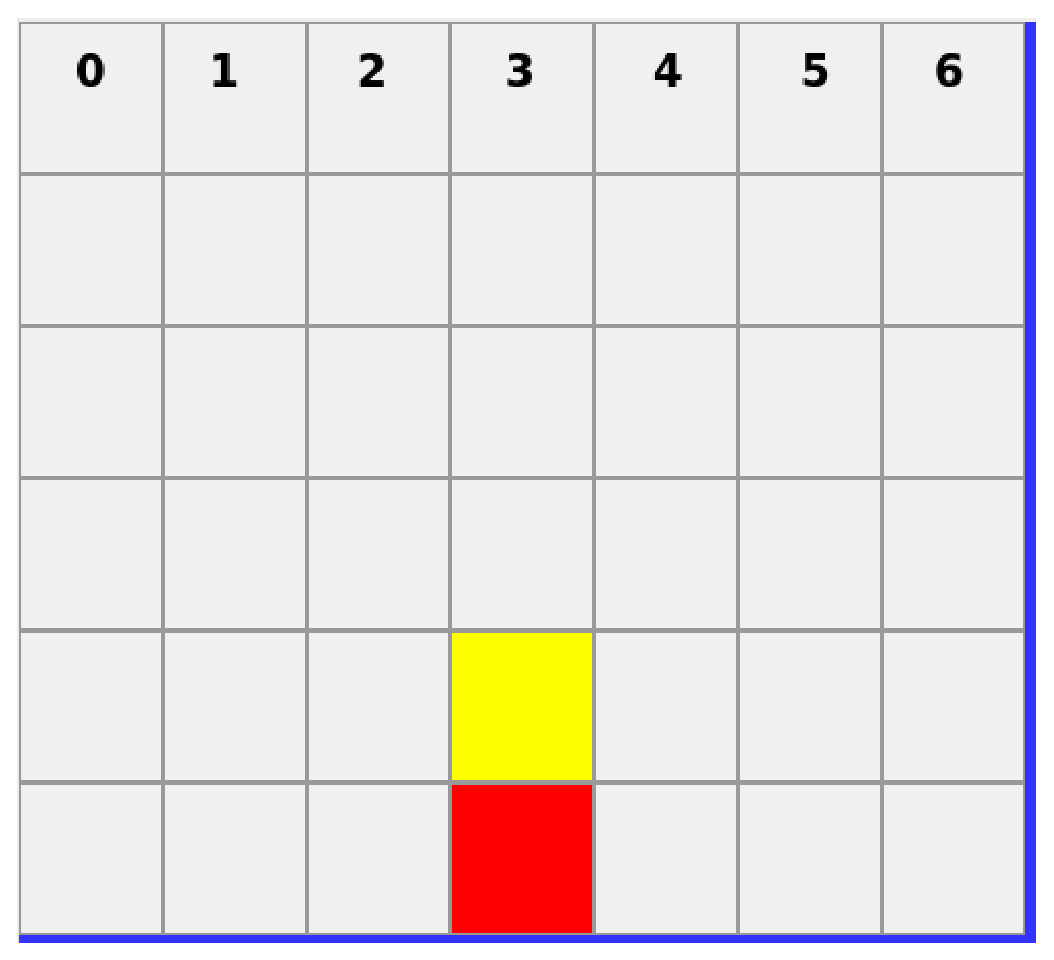
\includegraphics[scale=0.2]{playable0}
  \caption{\texttt{playable[i] = 0}}
\end{center}
\end{figure}
Dans ce cas, tous les playable[i] sont �gaux � 0. autrement dit on
peut jouer sur n'importe quelle case. Seulement notre intelligence
artificielle choisiera de jouer au centre du jeu, car la probabilit�
de gagner lors qu'on joue au centre est sup�rieure aux autres (par
exemple si on joue sur les cot�s).

\begin{figure}[H]
\begin{center}
  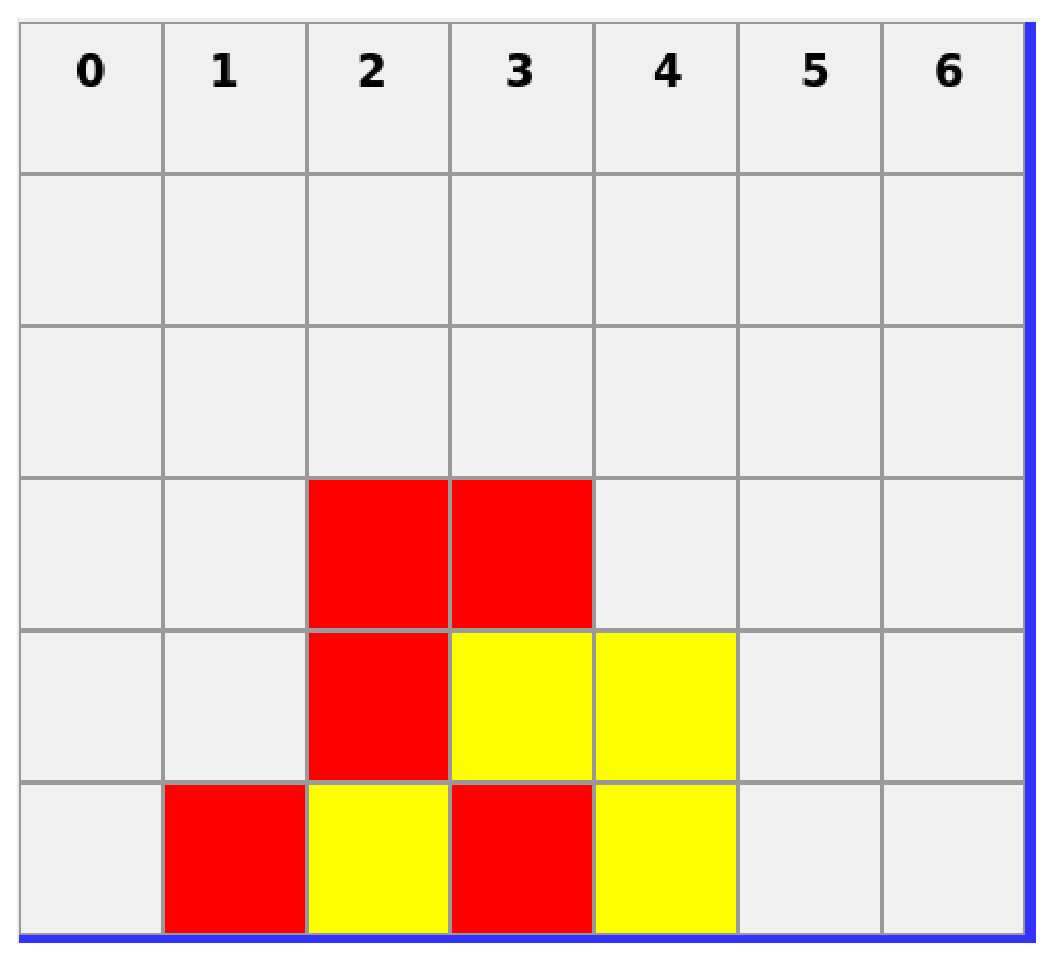
\includegraphics[scale=0.2]{playable10}
  \caption{\texttt{playable[i] = 1}}
\end{center}
\end{figure}
Si l'ordinateur joue sur la colonne 4, alors au prochain coups le
joueur humain pourra gagner avec une diagonale. Par cons�quent
\texttt{playable[4]=1}. Ce code signifie que si l'ordinateur joue sur
cette colonne alors cela peut faire gagner le joueur humain.

\begin{figure}[H]
\begin{center}
  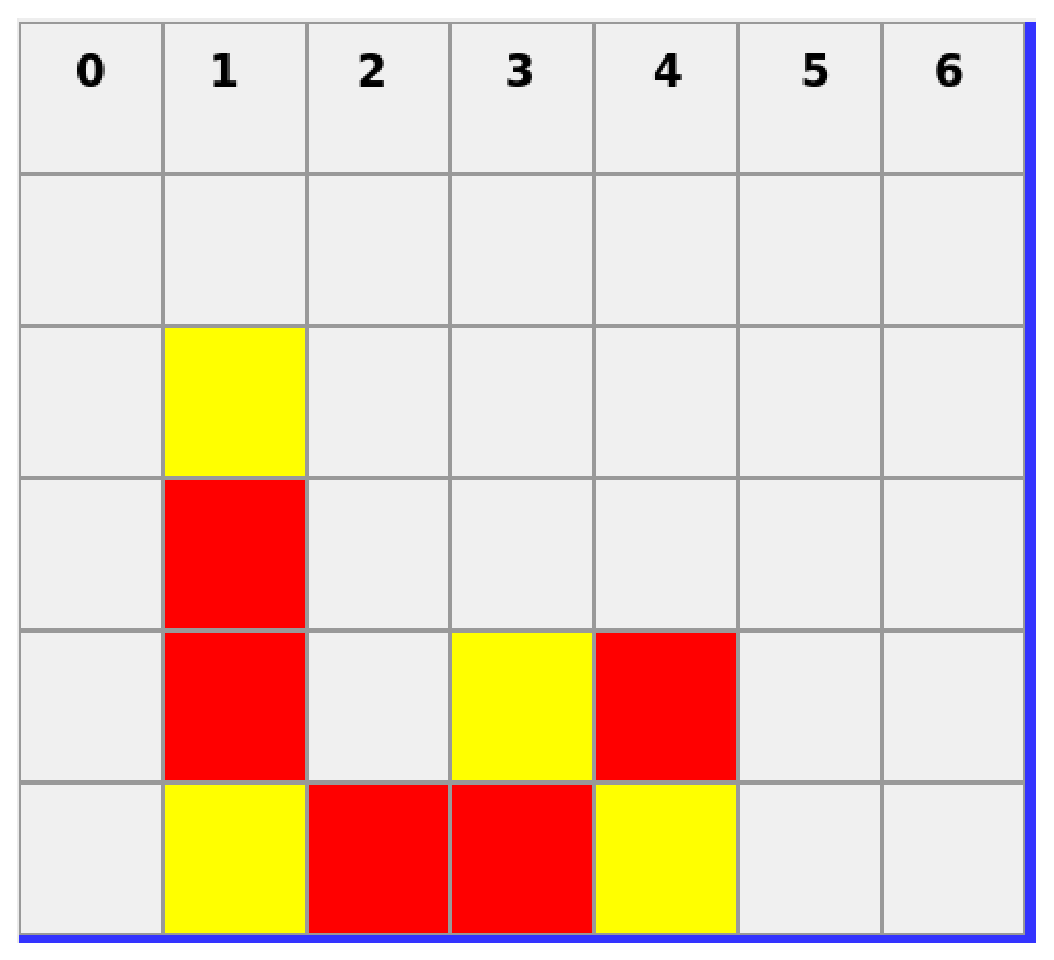
\includegraphics[scale=0.2]{playable2}
  \caption{\texttt{playable[i] = 2}}
\end{center}
\end{figure}
Dans ce cas \texttt{playable[2] = 2}. Autrement dit, si l'ordinateur
joue sur la colonne deux, le joueur humain pourra le bloquer.

\begin{figure}[H]
\begin{center}
  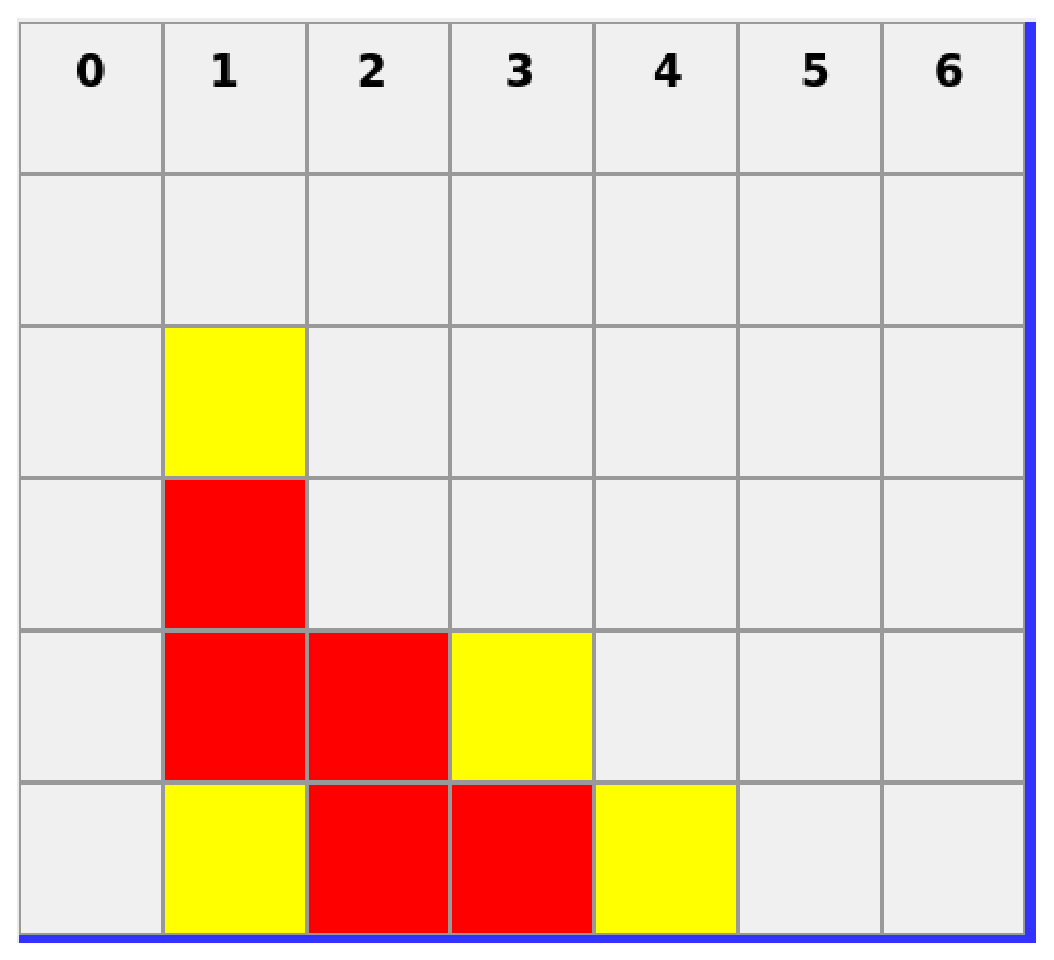
\includegraphics[scale=0.2]{playable3}
  \caption{\texttt{playable[i] = 3}}
\end{center}
\end{figure}
Dans ce cas \texttt{playable[2] = 3}. Par cons�quent l'ordinateur peut
gagner ua prochain coups, et jouera la position 2.

\begin{figure}[H]
\begin{center}
  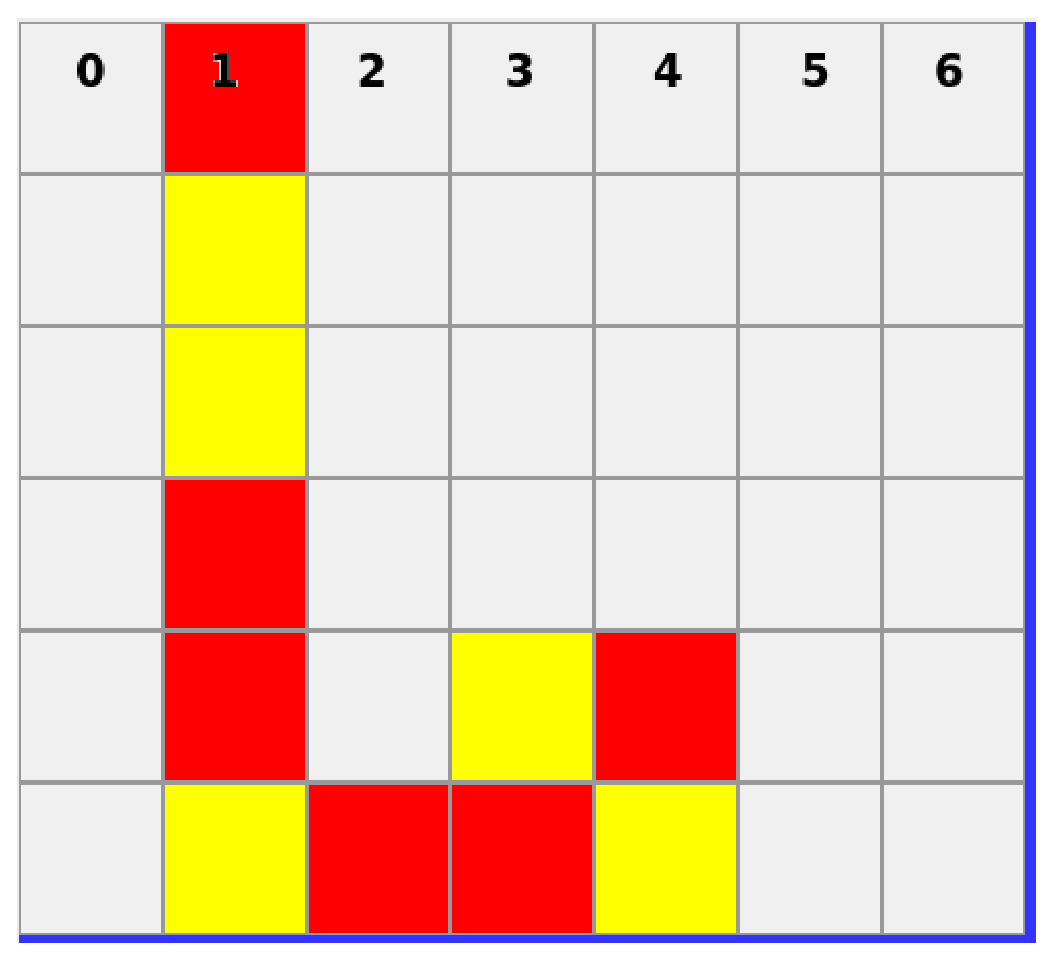
\includegraphics[scale=0.2]{playable4}
  \caption{\texttt{playable[i] = 4}}
\end{center}
\end{figure}
La colonne 1 est pleine donc \texttt{playable[1] = 4}. L'ordinateur
prend conscience qu'il ne pourra pas placer de jetons dans cette
colonne.

\begin{figure}[H]
\begin{center}
  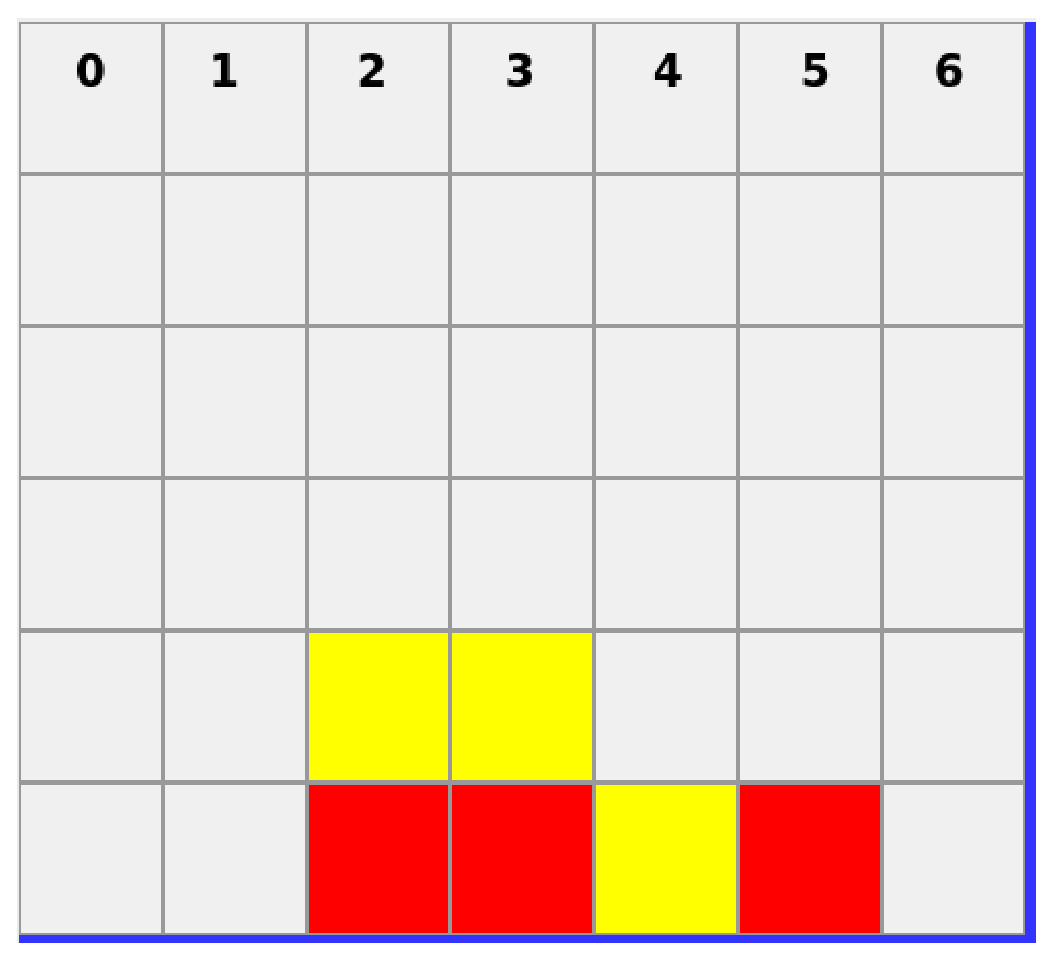
\includegraphics[scale=0.2]{playable5}
  \caption{\texttt{playable[i] = 5}}
\end{center}
\end{figure}
A ce moment du jeu, l'ordinateur remarque qu'il peut gagner en
ajoutant 2 pions. Par cons�quent il va marquer \texttt{playable[4] =
  5} et \texttt{playable[5] = 5}.


\begin{figure}[H]
\begin{center}
  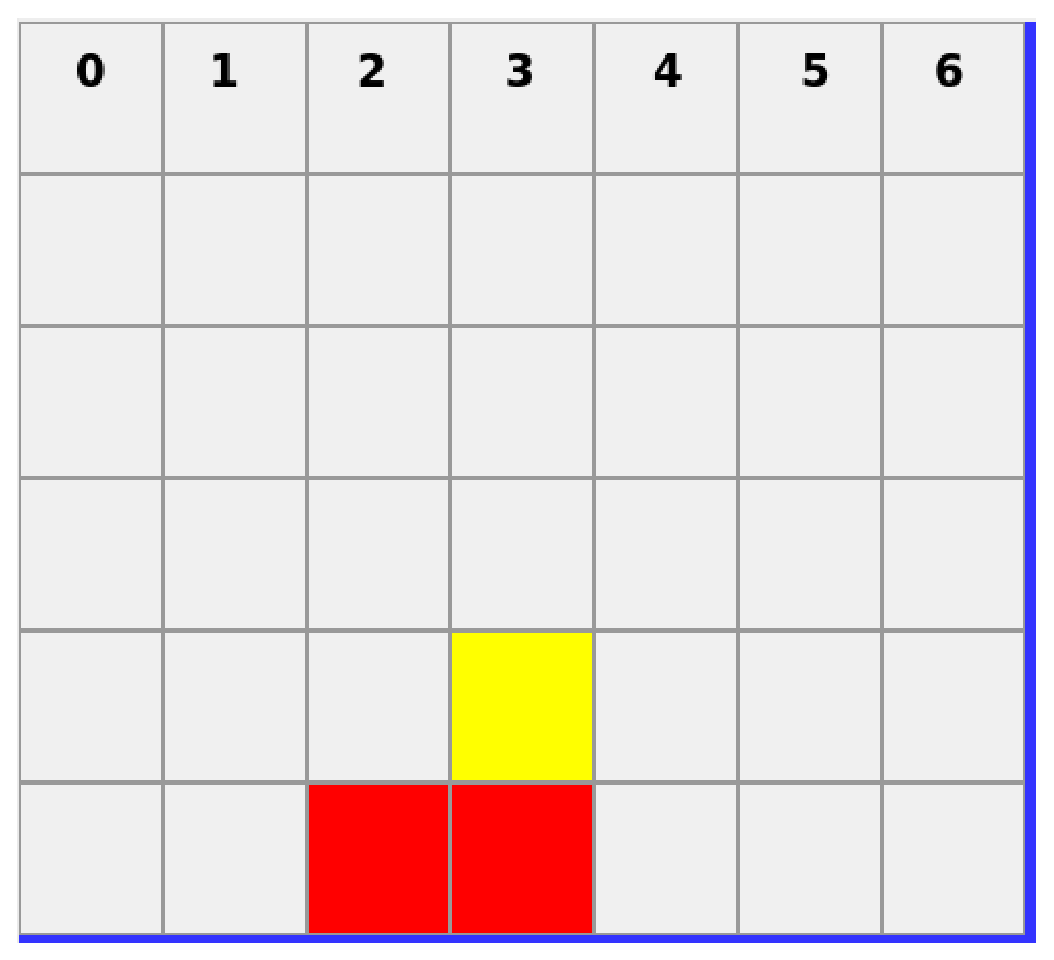
\includegraphics[scale=0.2]{playable1}
  \caption{\texttt{playable[i] = 6}}
\end{center}
\end{figure}
Dans ce cas la \texttt{playable[1] = 6} et \texttt{playable[4] = 6}. Et tous
les autres cas \texttt{playable[i]=0}. L'ordinateur va bloquer la
possibilit� de mouvement de l'humain.

\begin{figure}[H]
\begin{center}
  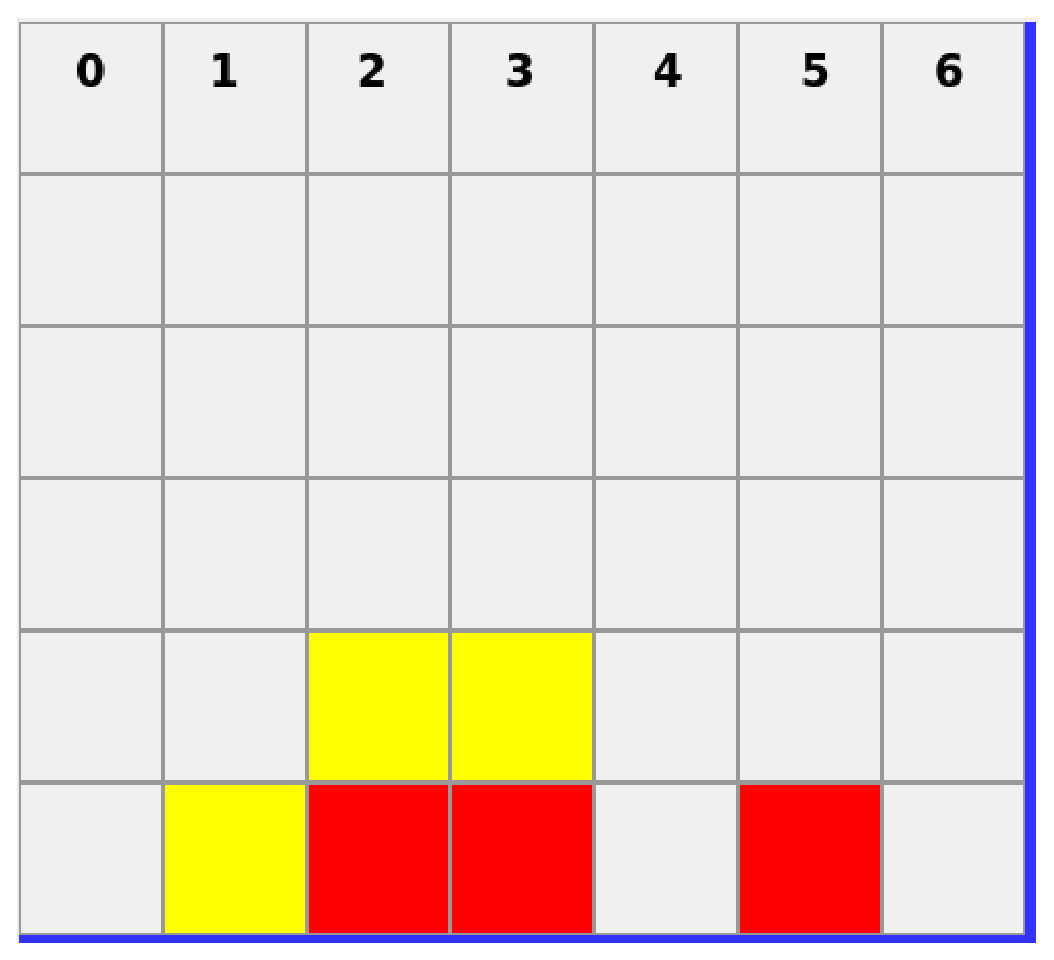
\includegraphics[scale=0.2]{playable6}
  \caption{\texttt{playable[i] = 6}}
\end{center}
\end{figure}
Si le joueur humain place un pion dans la colonne 4 il remportera la
victoire. Pour eviter de perdre aussi facilement on met
\texttt{playable[4]=6}, et l'ordinateur va bloquer la victoire du
joeur humain.

\begin{verbatim}
    private Rules rule;
    private int height;
    private int width;
\end{verbatim}
La premi�re variable va contenir les r�gles du jeu qui sont utilis�es,
dans notre cas ce sera pour le Puissance 4. Les deux variables
suivantes contiennent la hauteur, respectivement la largeur de notre \texttt{cpugrid}.

\begin{verbatim}
    private void strategy();
    private void breakStrategy();
    private void noPlayable();
    private void winningPlayable();
    private void fillPlayable();
\end{verbatim}
La m�thode \texttt{strategie()} va parcourir la grille et calculer les
positions que l'ordinateur peut jouer pour pouvoir gagner en deux
coups. une fois qu'elle a rep�rer les colonnes et remplie en
cons�quence \texttt{playable[i]}. La m�thode suivante,
\texttt{breakStrategy()} va parcourir la grille et va regarder si
lorsque l'ordinateur joue un coup, alors cela permettra a l'humain de
la bloquer alors qu'avant il ne le pouvait pas. (pour plus de d�tails
voir les captures d'�cran pr�c�demment). Dans ce cas
\texttt{playable[i] = 5}.

La m�thode \texttt{noPlayable} a un double usage. tout d'abord elle
regarde si le joueur humain peut gagner au prochain coups. Dans ce cas
elle marque \texttt{playable[i] = 6} (i correspondant � la
colonne). Mais elle va aussi v�rifier si en jouant une colonne cela
permet � l'humain, au coups d'apr�s, de gagner la partie. Dans ce cas
\texttt{playable[i] = 1}.

Pour \texttt{winningPlayable()}, on regarde si l'ordinateur peut
gagner au prochain coups, et on marque la colonne correspondante par 3
autrement dit \texttt{playable[i] = 3}.

La m�thode \texttt{fillPlayable()} quand a elle initialise
\texttt{playable[i] = 0} pour les colonnes ou on peut encore
jouer. Pour ce qui concerne les colonnes pleines, alors
\texttt{fillPlayable()} va mettre \texttt{playable[i]=4}.

\begin{verbatim}
    public void initialize(DataStructure grid, int difficulty);
    public int play(Rules new_rule);
\end{verbatim}
La m�thode \texttt{initialize()} n�st pas un constructeur, mais comme
son nom l'indique, elle va initialiser le \texttt{Cpu}. Quand � la
m�thode \texttt{play()} elle va v�rifier selon le \texttt{mode},
autrement dit la \texttt{difficulty}, quelle IA appeler.

\begin{verbatim}
    public int perfectCpu();
    public int easyCpu();
\end{verbatim}
Ces deux m�thodes sont tr�s similaires, � la diff�rence que le
\texttt{perfectCpu()} appelle les m�thodes \texttt{breakStrategy()} et
\texttt{strategy()}, ce que ne fais pas la m�thode
\texttt{easyCpu()}. Le mode \texttt{easyCpu} est moins agressif que le
mode \texttt{perfectCpu()}, qui en passant n'est pas parfait ;-)\newline
Dans notre m�thode \texttt{perfectCpu()} on commence par remplir la
grille avec \texttt{fillGrid()} et continue par v�rifier si
on peut gagner au prochain coup � l'aide de la m�thode
\texttt{winningPlayable()}. Si il y a une position gagnante alors on
retourne le num�ro de la colonne. Sinon on regarde si le joueur humain
peut gagner au prochain coups, ou si jouer une certaine colonne peut
le faire gagner. Tout cela � l'aide de la m�thode
\texttt{noPlayable()}.


Si on est dans le \texttt{perfectCpu()} alors on �tablie une
strat�gie. Pour cela on �vite de jouer une colonne ou l'humain
pourrait nous bloquer par la suite, avec la m�thode
\texttt{breakStrategy()}. Ensuite on essaie d'�tablir une strat�gie,
si on a 2 jetons align�s, alors on va essayer d�n aligner 2 de plus
pour faire un 4 � la suite, � l'aide de la m�thode
\texttt{strategy()}. Cela ne se fait que dans la m�thode \texttt{perfectCpu()}


On continue, peu importe la m�thode \texttt{perfectCpu()} ou
\texttt{easyCpu()}, on regarde si on a autre chose que des 0, 1 et 2
dans \texttt{playable[i]}, et dans ce cas on remplit les colonnes du
milieu de la grille. Sinon dans l'ordre des priorit�s pour
\texttt{playable[i]} l'ordinateur joue de cette mani�re : \texttt{3 -
  6 -  5 -  0 -  2 -  1}.

\subsubsection{Jeux de test}

TODO

\subsection{Rules}

\texttt{Rules} est une interface. Cela nous permet d'impl�menter de
nouvelles r�gles. Ca peut �tre utile si on veut transformer notre
Puissance 4 en Morpion, ou si on veut faire un Puissance 5 ...

\subsubsection{FourInARow}
Cette classe impl�mente \texttt{Rules}.

\begin{verbatim}
    public boolean checkDiag(int i, int j, int color, DataStructure grid);
    public boolean checkCol(int i, int j, int color, DataStructure grid);
    public boolean checkLine(int i, int j, int color, DataStructure grid);
    public boolean isComplete(DataStructure grid);
    public boolean checkPlay(int play, DataStructure grid);
    public void greyOut(GUI app, DataStructure grid);
\end{verbatim}

\texttt{checkDiag()} retourne \texttt{true} si il existe un alignement
de 4 jetons d'une m�me couleur en diagonale. Il retourne
\texttt{false} sinon. \texttt{checkCol()} retourne \texttt{true} si il existe un alignement
de 4 jetons d'une m�me couleur en colonne. Il retourne
\texttt{false} sinon. \texttt{checkLine()} retourne \texttt{true} si il existe un alignement
de 4 jetons d'une m�me couleur en Ligne. Il retourne
\texttt{false} sinon. \texttt{isComplete()} va faire appel aux trois
m�thodes pr�c�dentes afin de v�rifier si il y a un gagnant. Auquel cas
cette m�thode retourne \texttt{true}, sinon elle renvoie
\texttt{false}. La m�thode \texttt{checkPlay()} v�rifie que la
position pass�e en argument est jouable, elle renvoie \texttt{true} si
c�st jouable, et \texttt{false} sinon.

La derni�re m�thode, \texttt{greyOut()}, va quand a elle griser les bouttons des colonnes
pleines correspondantes.

\subsubsection{Tests de FourInARow}
Cette classe teste :\newline 
\begin{itemize}


\item L'existence ou non d'un alignement de 4 jetons d'une m�me couleur soit dans la m�me ligne, m�me colonne, m�me diagonale :\newline
On choisit des valeurs al�atoires valides (constituant une : ligne, colonne, diagonale) afin de v�rifier le comportement de nos m�thodes d'alignement des jetons.\newline
Exemple (Existence de 4 jetons sur la m�me ligne) :\newline
On cr�e 4 jetons sur la m�me ligne 0:
\begin{center}
\textbf{assertTrue(matrix.setValue(0, 0, 1));}\newline
\textbf{assertTrue(matrix.setValue(0, 1, 1));}\newline
\textbf{assertTrue(matrix.setValue(0, 2, 1));}\newline
\textbf{assertTrue(matrix.setValue(0, 3, 1));}\newline
\end{center}

Puis en bouclant sur toutes les positions de la grille, on arrive � effectuer un test complet sur l'existence ou non d'un alignement de 4 jetons sur une ligne donn�e.\newline

\item Qu'une position donn�e est jouable en remplissant la grille al�atoirement mais de mani�re � ce qu'une position soie jouable/non jouable.  

\end{itemize}

\subsection{GameEngine}
\subsubsection{Impl�mentation}
\begin{verbatim}
    private DataStructure grid;
    private boolean current_player;
    private int currently_played;
    private GUI app;
    private int mode;
    private Rules rule;
    private Player player1;
    private Player player2;
    private int counter;
\end{verbatim}
La variable \texttt{grid} contient la grille du
jeu. \texttt{current\_player} peut obtenir deux valeurs, 0 qui
correspond au joueur 1, et 1 qui correspond au joueur
2. \texttt{currently\_played} contient le coup jou� (une position ou un
reset). \texttt{app} contient l'interface graphique. \texttt{mode}
contient le mode de jeu. \texttt{rule} contient les r�gles du
jeu. \texttt{playerX} contient le joueur, qui peut etre humain ou
artificiel. \texttt{counter} contient le nombre de coups jou�, cela
nous permet de d�terminer si il y a un match nul.

\begin{verbatim}
    public GameEngine();
    public void initMode(int my_mode);
    public void close();
    public void start();
    public void resetGrid();
    public void updatePlay();

    private void updateGrid();
\end{verbatim}
Le constructeur initialise l'interface graphique, la grille (avec une
taille que l'on peut modifier) et les r�gles du jeu. La m�thode
\texttt{initMode()} initialise les joueurs, la variable
\texttt{my\_mode} et reset le \texttt{counter}. La m�thode
\texttt{close()} quand � elle ferme l'interface graphique. Cette
m�thode n'est appel�e que par le \texttt{Main()}.

La m�thode \texttt{start()} s'occupe de lancer le jeu. il aura �t�
initialis� par les autres m�thodes qui la pr�c�de.\newline
La boucle \texttt{while((!rule.isComplete(grid)) \&\& (counter <} 
\texttt{grid.getWidth() * grid.getHeight()))} va faire en sorte que le jeu
ne se termine pas tant qu'il n'y a pas de gagnant ou que la grille
n'est pas pleine. Il faut savoir que l'utilisateur peut arr�ter le
programme a tout moment a l'aide de l'interface graphique.

Cette m�thode fiat jouer a tour de r�le le joueur 1 et le joueur
2. C'est la m�thode \texttt{start()} qui va interpr�ter le choix du
joueur, autrement dit, si \texttt{currently\_played = -2} ca implique
qu'il faut reset la grille.

A chaque tour de boucle on incr�mente la variable \texttt{counter} de
un si la position jou�e est valide. Par la suite on met � jour la
grille � l'aide de la m�thode \texttt{updatePlay()} et on grise les
bouttons dont les colonnes sont pleines � l'aide de la m�thode
\texttt{rule.greyOut()}.

Une fois la boucle termin�e, autrement dit, lorsque le jeu est termin�
on v�rifie qui a gagn� et on l'affiche � l'aide de la m�thode \texttt{gameEnded()}.

La m�thode \texttt{resetGrid()} s'occupe d'initialiser la
\texttt{grid} avec des 0, elle fait en sorte de ne aps re-faire
appelle � elle avec la m�thode \texttt{app.setReset(false)} et
r�initialise tous les boutons avec la m�thode
\texttt{app.enableAllButton()}. Il faut aussi r�initialiser le
\texttt{counter} et mettre � jour l'affichage graphique.

La m�thode \texttt{updatePlay()}, va quand � elle, re-v�rifier si la
position jou�e est valide puis va mettre � jour la grille, et enfin
met � jour l'affichage.

La m�thode \texttt{updateGrid()} va mettre � jour la grille, autrement
c�st elle qu iva g�n�rer la gravit�, si on peut dire.

\subsubsection{Tests du GameEngine}
Pour valider le fonctionnement du GameEngine qui s'av�re d�licat � tester correctement
avec JUnit nous avons choisis une autre approche. Nous avons cr�e une
classe IARandom qui va nous servir uniquement � tester de mani�re
al�atoire le fonctionnement de notre moteur de jeu. Cette IA tire au
sort une colonne et joue un pion dans cette colonne si le coup est
valide sinon elle tire de nouveau une colonne au sort.



\subsection{Main et Menu}
Le \texttt{Main()} va instancier le \texttt{GameEngine} mais aussi le
menu de d�part. c�st le \texttt{Main()} qui va dire au
\texttt{Gameengine} de d�marrer le jeu avec l'appel � la m�thode
\texttt{g.start()}. Le \texttt{Main()} fait au \texttt{GameEngine}
instancier les joueurs avec l'appel � la m�thode
\texttt{g.initMode(my\_menu.choice)}.\newline
\newline
Pour ce qui concerne le menu, on aurait pu l'int�grer dans l'interface
graphique, mais nous n'avions pas assez de temps pour faire cette
petite modification, et nous avons pr�f�r� passer aux tests directement.

\subsection{GUI}

\texttt{GUI} est une interface, cela nous permettra, au besoin, de branher une autre interface graphique � notre application.

\subsubsection{GuiOwn}
Cette classe, impl�mente \texttt{GUI}. 
\begin{verbatim}
    public int choice;
    public boolean played;
    public boolean reset;
    public boolean game_ended;
\end{verbatim}
La premi�re variable \texttt{choice} contient la colonne s�lectionn� par le joueur humain. La seconde variable \texttt{played} est a \texttt{true} lorsqu'un joueur a choisi une colonne et est a \texttt{false} sinon. Il en est de m�me pour \texttt{reset} et pour \texttt{game\_ended}. A savoir que \texttt{reset} concerne le reset de la grille et \texttt{game\_ended} dit si le jeu est termin� ou non.

\begin{verbatim}
    public abstract void initGui(DataStructure grid);
\end{verbatim}
Cette m�thode initialise l'interface grapique en cr�ant autant de colonne et de ligne que la matrice en a.

\begin{verbatim}
    public abstract void updateScreen(DataStructure my_grid);
\end{verbatim}
\texttt{updateScreen} met a jour l'affichage de la grille.

\begin{verbatim}
    public abstract void gameEnded(boolean winner);
    public abstract void gameEnded();
\end{verbatim}
La premi�re m�thode affichage le nom du joueur dans l'interface graphique, et la seconde affiche Match nul.

\begin{verbatim}
    public abstract void greyAllButton();
\end{verbatim}
Cette m�thode grise tous les bouttons qui permettent de choisir les colonnes mais aussi de faire un reset de la grille. Elle est utilis� lorsque le jeu est termin�.

\begin{verbatim}
    public abstract void enableAllButton();
\end{verbatim}
Cette m�thode rend tous les bouttons correspondant aux colonnes non-gris�s. Elle est utilis� lors d'un reset.

\begin{verbatim}
    public abstract void greyButton(int num);
\end{verbatim}
\texttt{greyButton()} grise le boutton de la colonne correspondante � num.

\begin{verbatim}
    public void setSize(int i, int j);
    public void setLocation(int i, int j);
    public void show();
    public abstract void dispose();
\end{verbatim}
La premi�re m�thode permet de d�finir la taille de la fen�tre de jeu. La seconde sert � d�finir la position de la fen�tre par d�faut. La troisi�me est une m�thode d�finit dans les librairies de \texttt{Swing} qui permet d'afficher l'interface graphique. Quand � la derni�re m�thode, elle permet de d'afficher/fermer une fen�tre. La m�thode \texttt{dispose()} est aussi d�finit dans els librairies de \texttt{Swing}.

\begin{verbatim}
    public boolean getPlayed();
    public int getChoice();
    public void setPlayed(boolean played);
    public boolean getReset();
    public void setReset(boolean reset);
\end{verbatim}
Ces trois m�thodes sont de simples accesseurs aux variables correspondantes.


\newpage
% -*- mode: latex; coding: latin-1-unix -*- %

\section{Analyse Statique} 

Nous avons dans cette partie repr�sent� des fonctions cl�s de notre
programme � l'aide de CFA. Ceux-ci nous servent � effectuer une
s�rie de tests statiques des fonctions critiques du puissance4. Nous
trouverons dans l'ordre la fonction principale de notre moteur de jeu,
puis dans une seconde partie les CFA repr�sentant la partie IA du programme. 

Pour plus de clart� les deux CFA principaux que sont \texttt{start} et
\texttt{IA} sont amput�s des fonctions auquel ils font appel. On consid�rera d�s
lors que ces appels effectuent la fonctions pour lesquel ils sont
�crits et ne provoquent pas de bug du programme. Ces fonctions sont
repr�sent�es par la suite et sont analys�es s�par�ment. Dans cette
partie tous les tests sont effectu�s en bo�te blanche.
\subsection{GameEngine}

\begin{figure}[h]
\begin{center}
  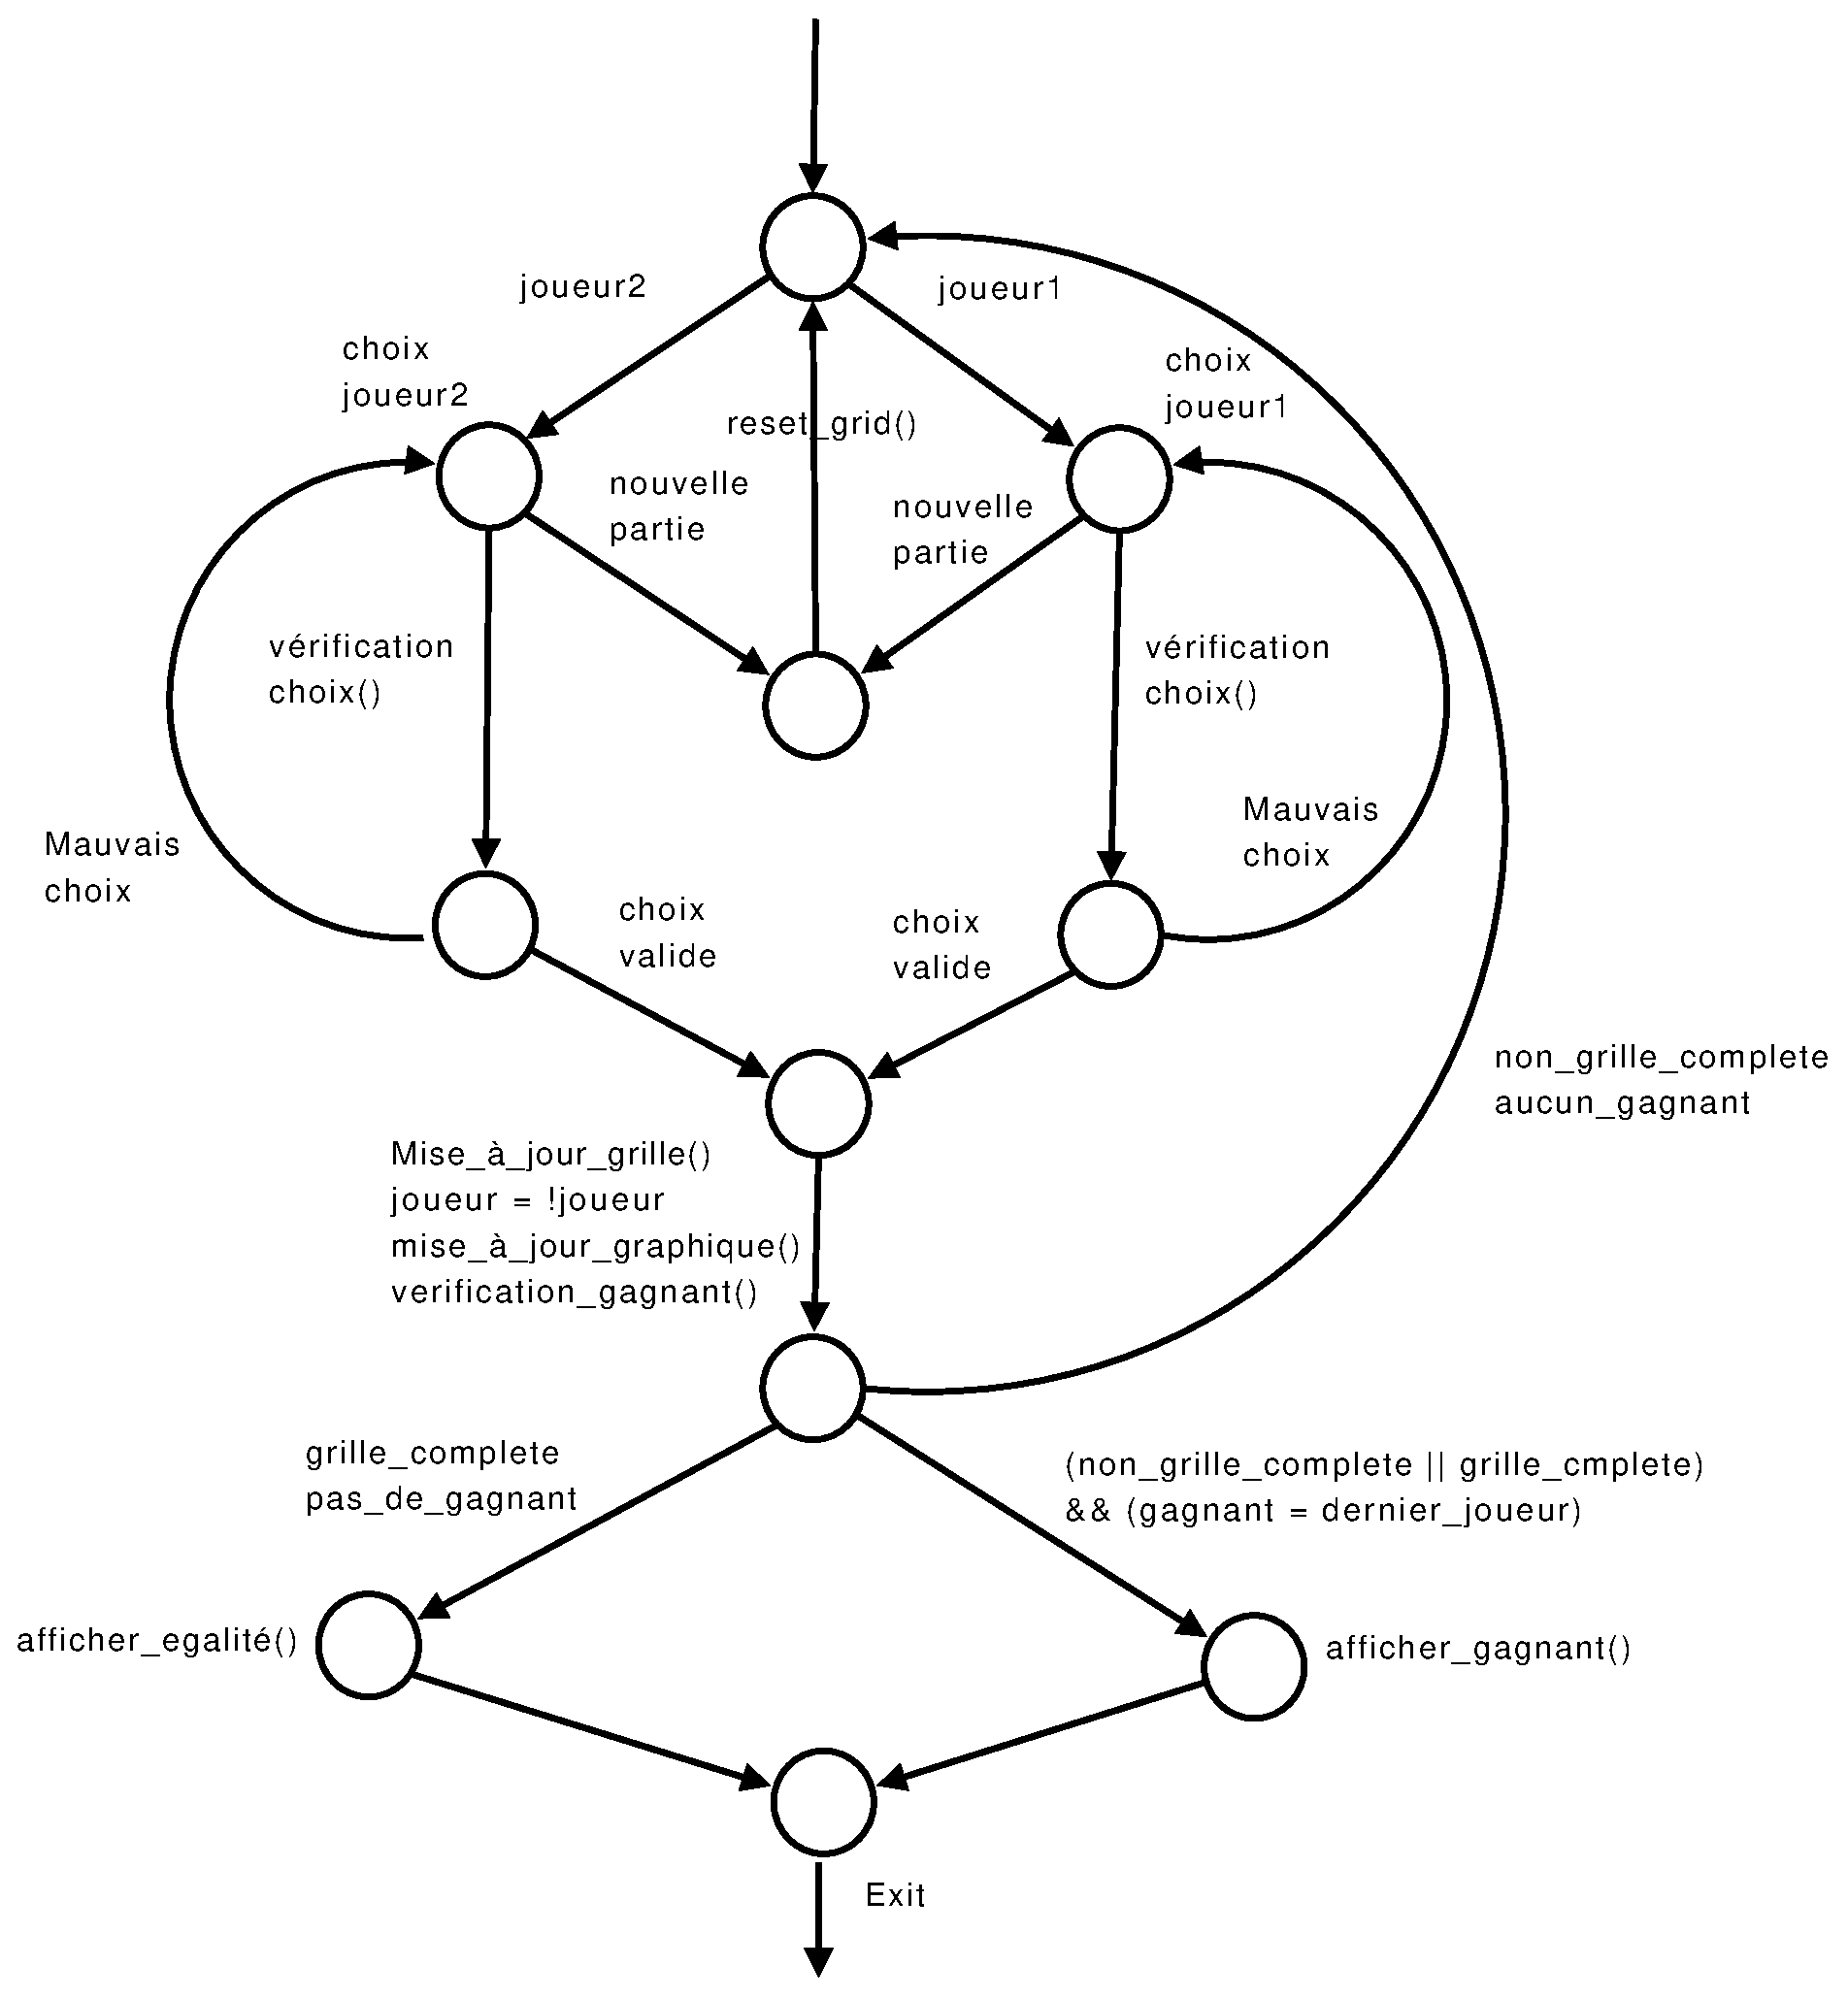
\includegraphics[scale=0.5]{start}
  \caption{Fonction start}
\end{center}
\end{figure}

\newpage

DT1=\{joueur1,joueur2,0=<choixJoueur1=<6,0=<choixJoueur2=<6,grille\_vide\}
En supposant qu'aucun des deux joueurs ne r�initialise la partie, et
que celle-ci ce termine, nous obtenons deux chemins possible :\\
\{0-2-5-6-7-0-3-4-6-7-...-9-10\} // partie avec un gagnant \\
\{0-2-5-6-7-0-3-4-6-7-...-8-10\} // partie avec un match nul\\

En prenant comme crit�re de couverture l'ensemble de tous les noeuds
nous obtenons un TER 1 = 9/11 = 81\%.\\

DT2=\{joueur1,joueur2,choixJoueur1=al�atoire,choixJoueur2=al�atoire,grille\_vide\}\\

Si un des deux joueurs � un moment donn� r�initialise la partie nous
obtenons :\\
\{0-2-5-6-7-0-3-4-6-7-...-0-2-1-0-...-9-10\}\\
\{0-2-5-6-7-0-3-4-6-7-...-0-2-1-0-...-8-10\}\\

En prenant le m�me crit�re de couverture on a TER1=10/11= 90\%;

\subsubsection{Les fonctions}
\texttt{v�rification\_choix()}\\
\begin{figure}[h]
\begin{center}
  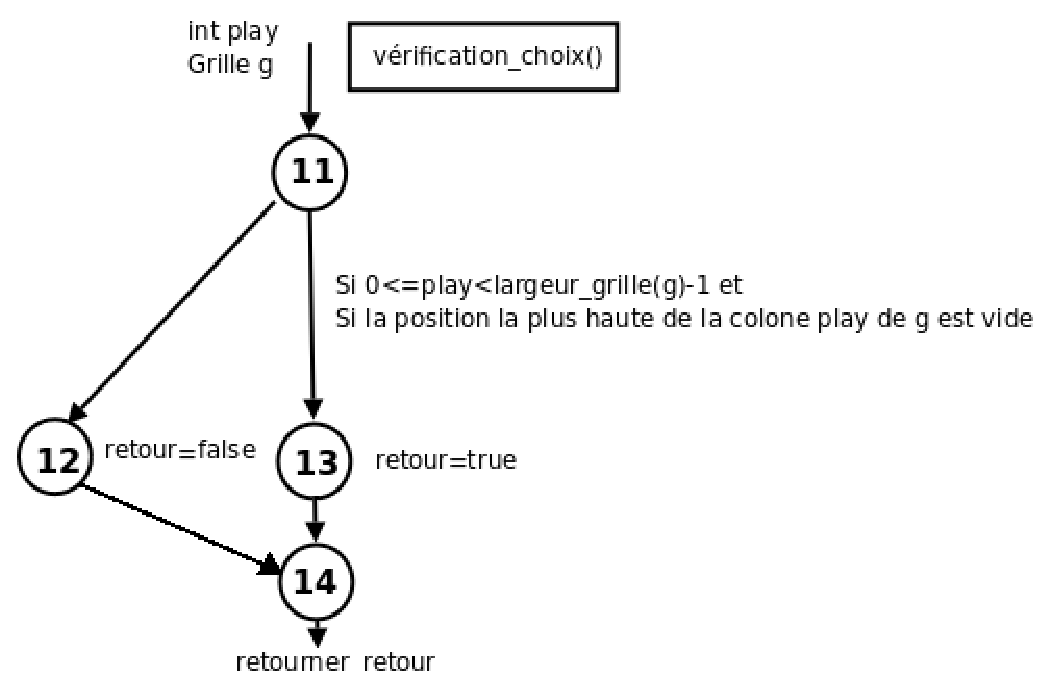
\includegraphics[scale=0.6]{verification_choix}
  \caption{Fonction v�rification choix}
\end{center}
\end{figure}

Cette fonction doit retourner un bool�en servant � savoir si la valeur
jou�e est comprise entre les valeurs de la grille et si la colone dans
laquel on veut jouer est pleine.\\

DT1=\{0=<play=<6,grille\_vide\}\\
DT2=\{0=<play=<6,grille\_pleine\}\\
DT3=\{play=9,grille\_vide\}\\

Si nous prenons toujours le crit�re de couverture de l'ensemble de
tous les noeuds, nous obtenons :\\


DT1 : TER1=3/4 = 75\% \{11-13-14\}\\
DT2 : TER1=3/4 = 75\% \{11-12-14\}\\
DT3 : TER1=3/4 = 75\% \{11-12-14\}\\



\texttt{v�rification\_gagnant()}\\
\begin{figure}[h]
\begin{center}
  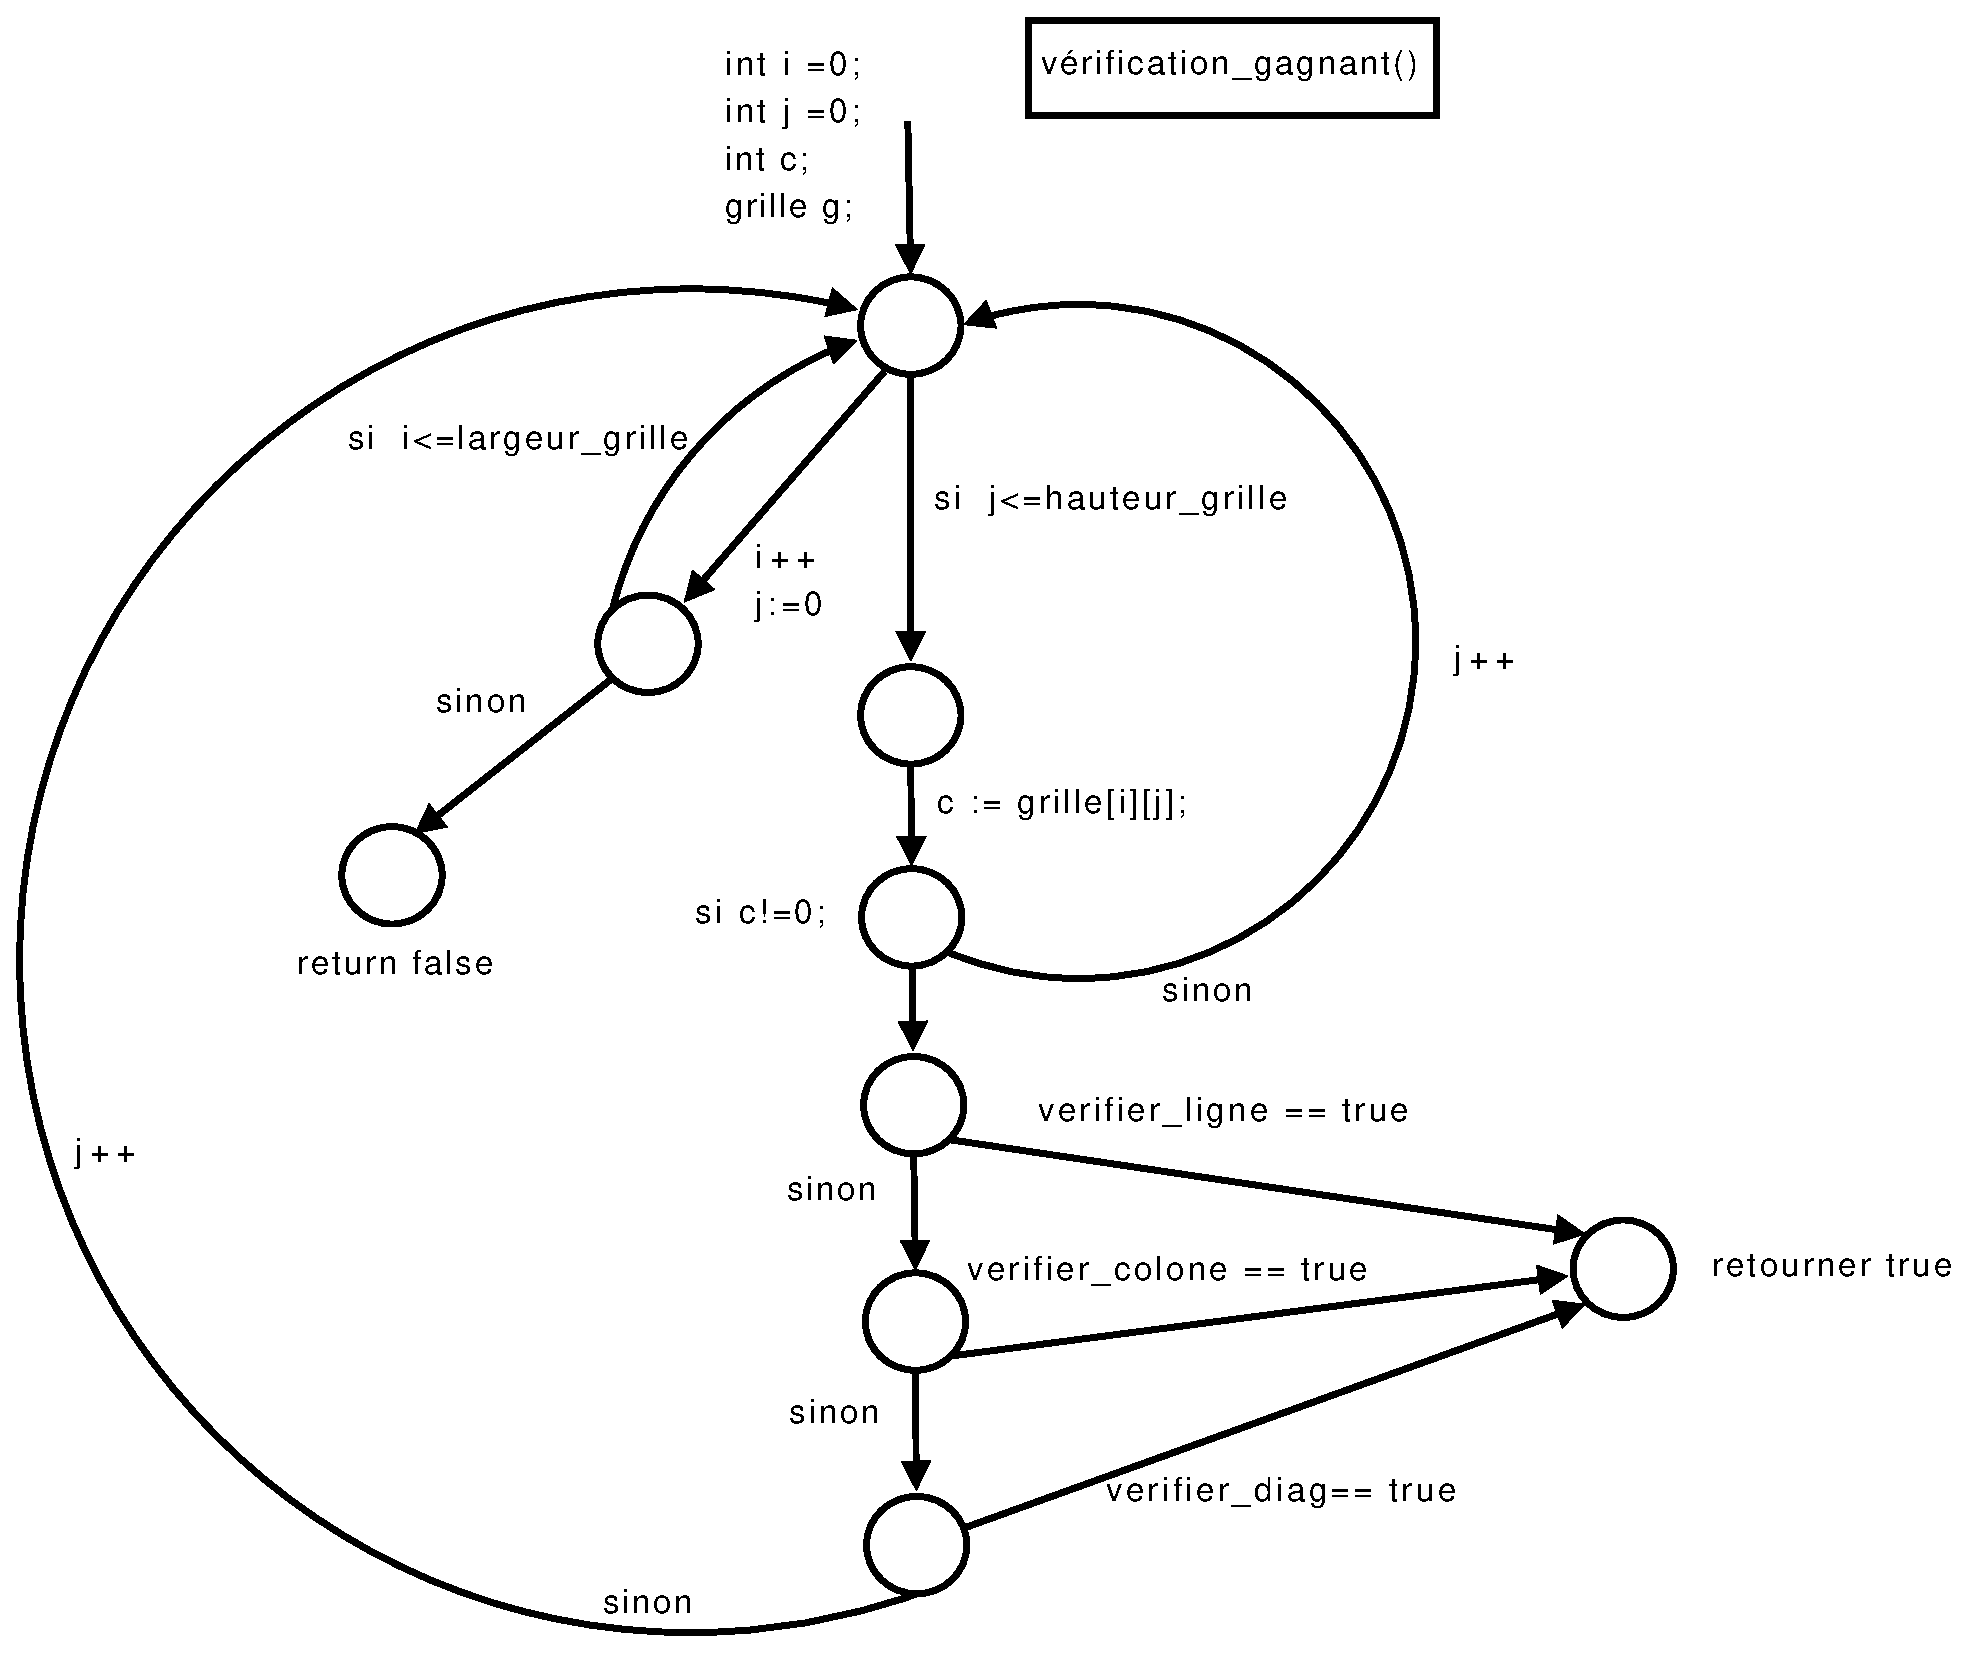
\includegraphics[scale=0.7]{verification_gagnant}
  \caption{Fonction v�rification gagnant}
\end{center}
\end{figure}

\newpage
Pour ce CFA si dans les DT il exite une ligne gagnante, une colone
gagnante ou une diagonale gagnante, on admetra que l'assertion dans le
programme retourne true.

DT1=\{grille\_en\_cours\_ de\_ partie,ligne\_gagnante\}\\
DT2=\{grille\_en\_cours\_ de\_ partie,colone\_gagnante\}\\
DT3=\{grille\_en\_cours\_ de\_ partie,diagonale\_gagnante\}\\
DT4=\{grille\_en\_cours\_ de\_ partie,pas\_de\_gagnant\}\\

DT1=\{15-16-16-15-18-15-16-17-...-20-21\}\\
DT2=\{15-16-16-15-18-15-16-17-...-20-22-21\}\\
DT3=\{15-16-16-15-18-15-16-17-...-20-22-23-21\}\\
DT4=\{15-16-16-15-18-15-16-17-...-15-18-19\}\\

Crit�re de couverture : L'ensemble des sommets du graphe.

DT1 : TER1=6/9=66\%\\
DT2 : TER1=7/9=77\%\\
DT3 : TER1=8/9=88\%\\
DT4 : TER1=5/9=55\%\\


\newpage
\subsection{IA}

Dans cette partie nous avons seulement mod�lis� le CFA de l'IA en mode
difficile car celui de l'IA facile est le m�me � la diff�rence pr�s de
ne pas comporter les fonction startegy et breakStrategy.

\begin{figure}[h]
\begin{center}
  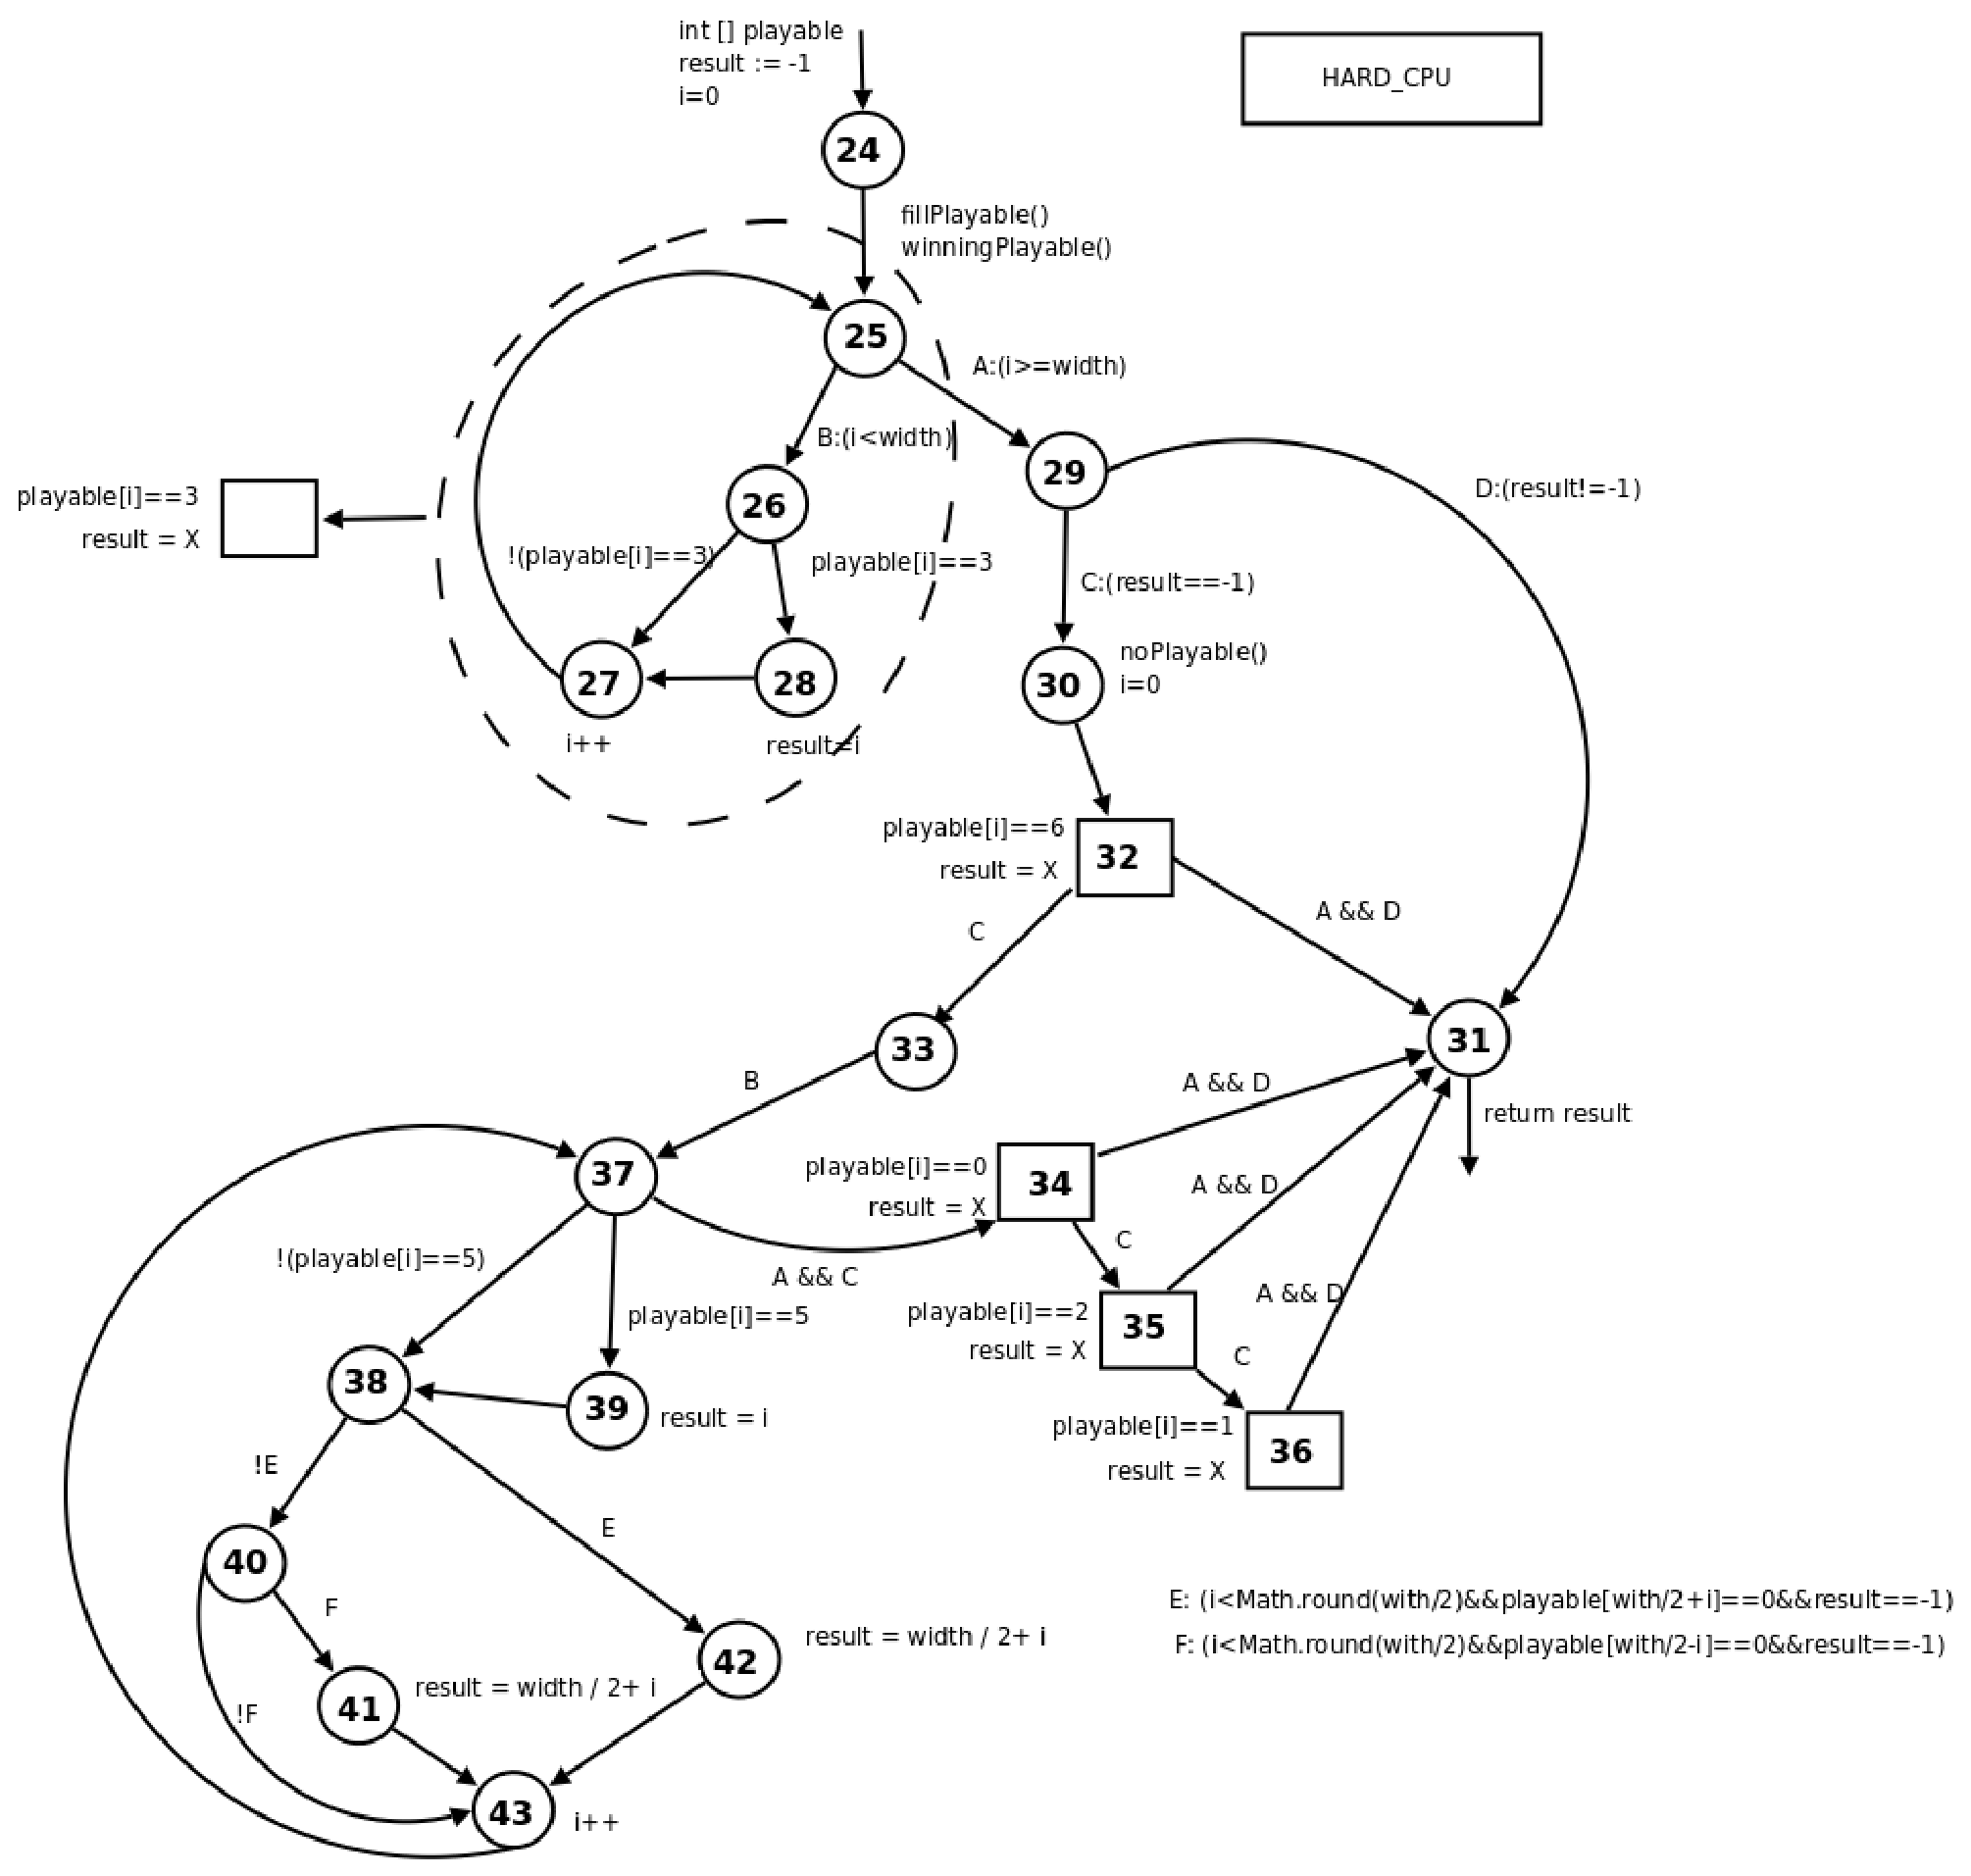
\includegraphics[scale=0.5]{IA}
  \caption{IA du programme}
\end{center}
\end{figure}

DT1=\{grille\_vide\}\\
DT2=\{grille\_pleine\_1\_position\_libre\}\\

DT1=\{24-25-26-27-25-29-31\}\\
DT2=\{24-25-26-28-27-25-29-30-32-31\}\\

Crit�re de couverture : L'ensemble des sommets du graphe.

DT1 : TER1= 21\%\\
DT2 : TER1= 31\%\\



\subsubsection{Les fonctions}
\texttt{fillPlayable()}\\
\begin{figure}[h]
\begin{center}
  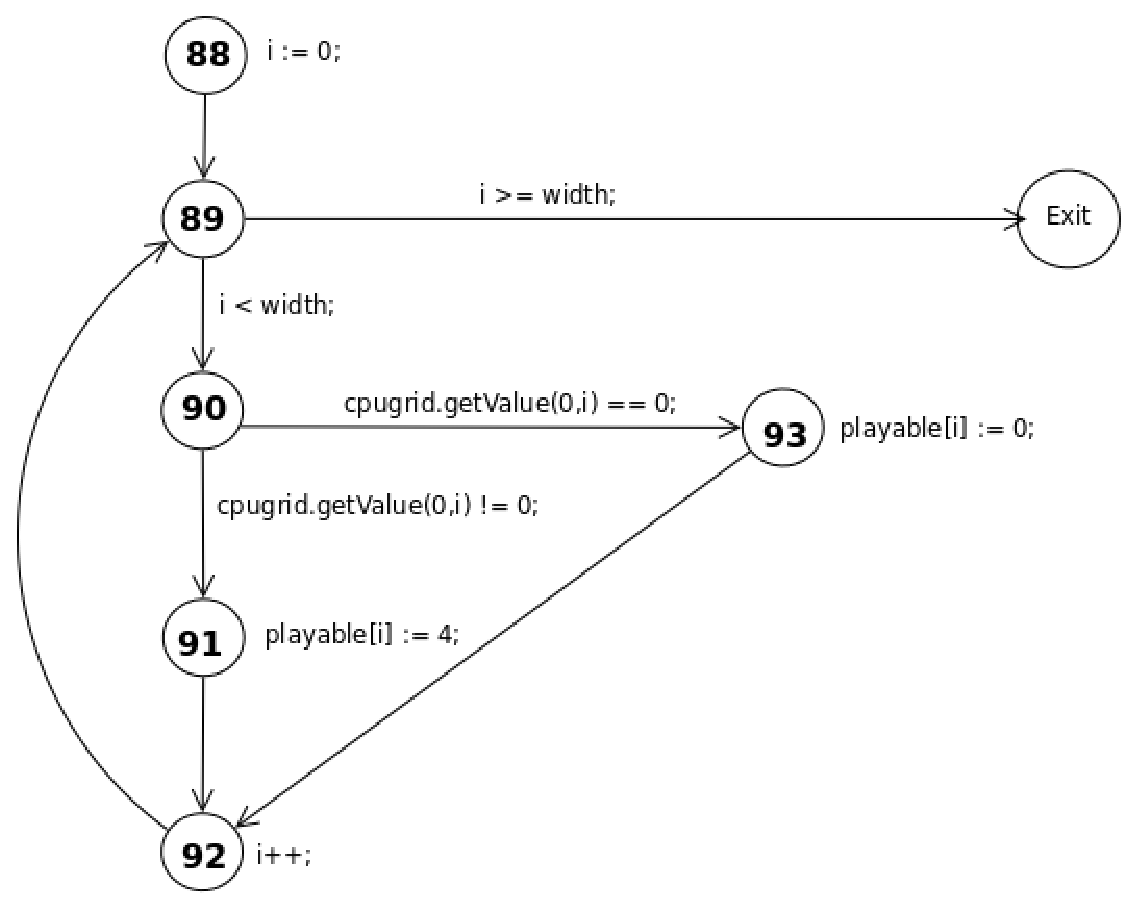
\includegraphics[scale=0.6]{fillPlayable}
  \caption{Fonction fillPlayable}
\end{center}
\end{figure}

DT1=\{grille\_vide\}\\
DT2=\{grille\_remplie\_avec\_positions\_libres\}\\

DT1=\{88-89-90-93-92-89-...-89-exit\}\\
DT2=\{88-89-90-93-92-89-...-89-90-91-92-89-exit\}\\

Crit�re de couverture : L'ensemble des sommets du graphe.

DT1 : TER1= 85\%\\
DT2 : TER1= 100\%\\


\newpage
\texttt{winningPlayable()}\\
\begin{figure}[h]
\begin{center}
  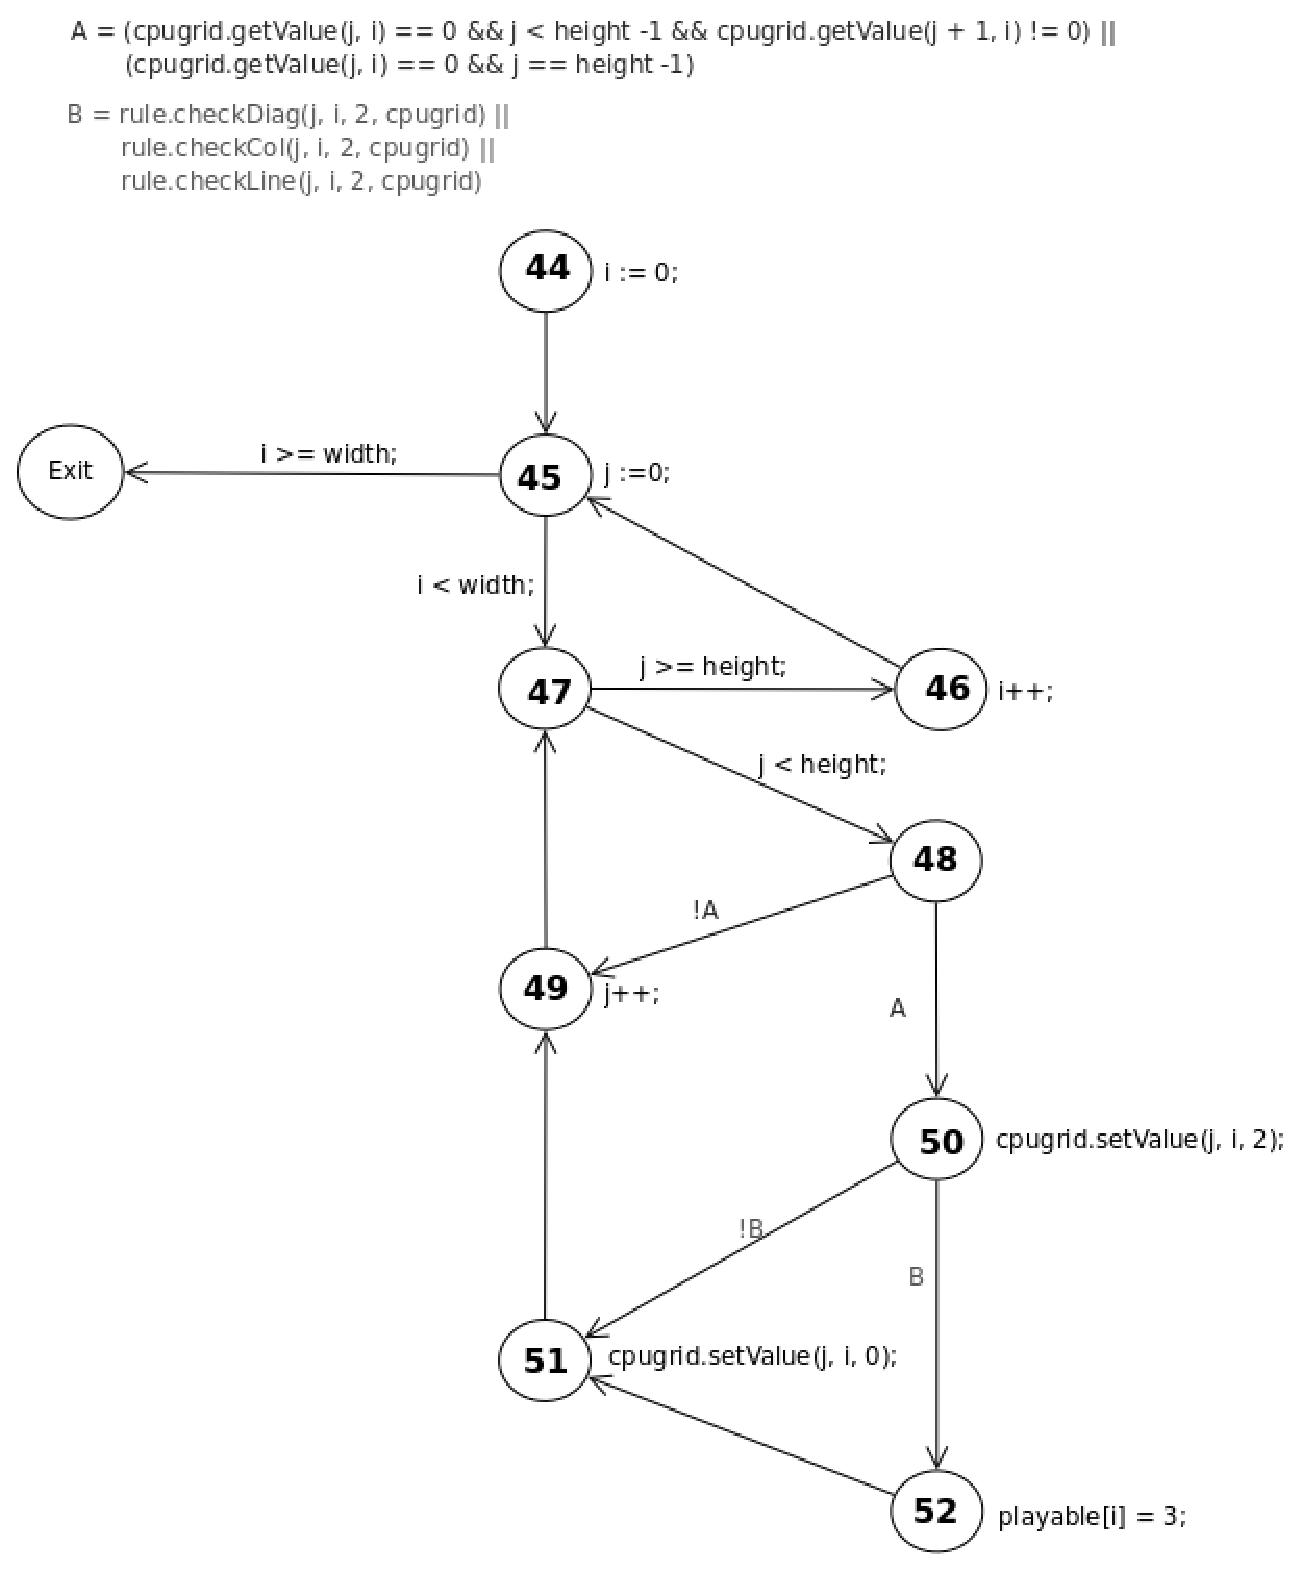
\includegraphics[scale=0.6]{winningPlayable}
  \caption{Fonction winningPlayable}
\end{center}
\end{figure}

DT1=\{grille\_vide\}\\
DT2=\{grille\_remplie\_avec\_positions\_libres\}\\

DT1=\{44-45-47-48-50-52-51-49-47-...-46-45-exit\}\\
DT2=\{44-45-47-48-49-47-...-46-45-exit\}\\

Crit�re de couverture : L'ensemble des sommets du graphe.

DT1 : TER1= 100\%\\
DT2 : TER1= 70\%\\

Pour les 3 derniers CFA nous n'avons pas trouv� de DT suffisament
pertinentes pour �tre int�gr�s dans le rapport. Nous les avons
n�anmoins fournis en consultation dans les pages suivantes.\\ 

\texttt{noPlaybale()}\\
\begin{figure}[h]
\begin{center}
  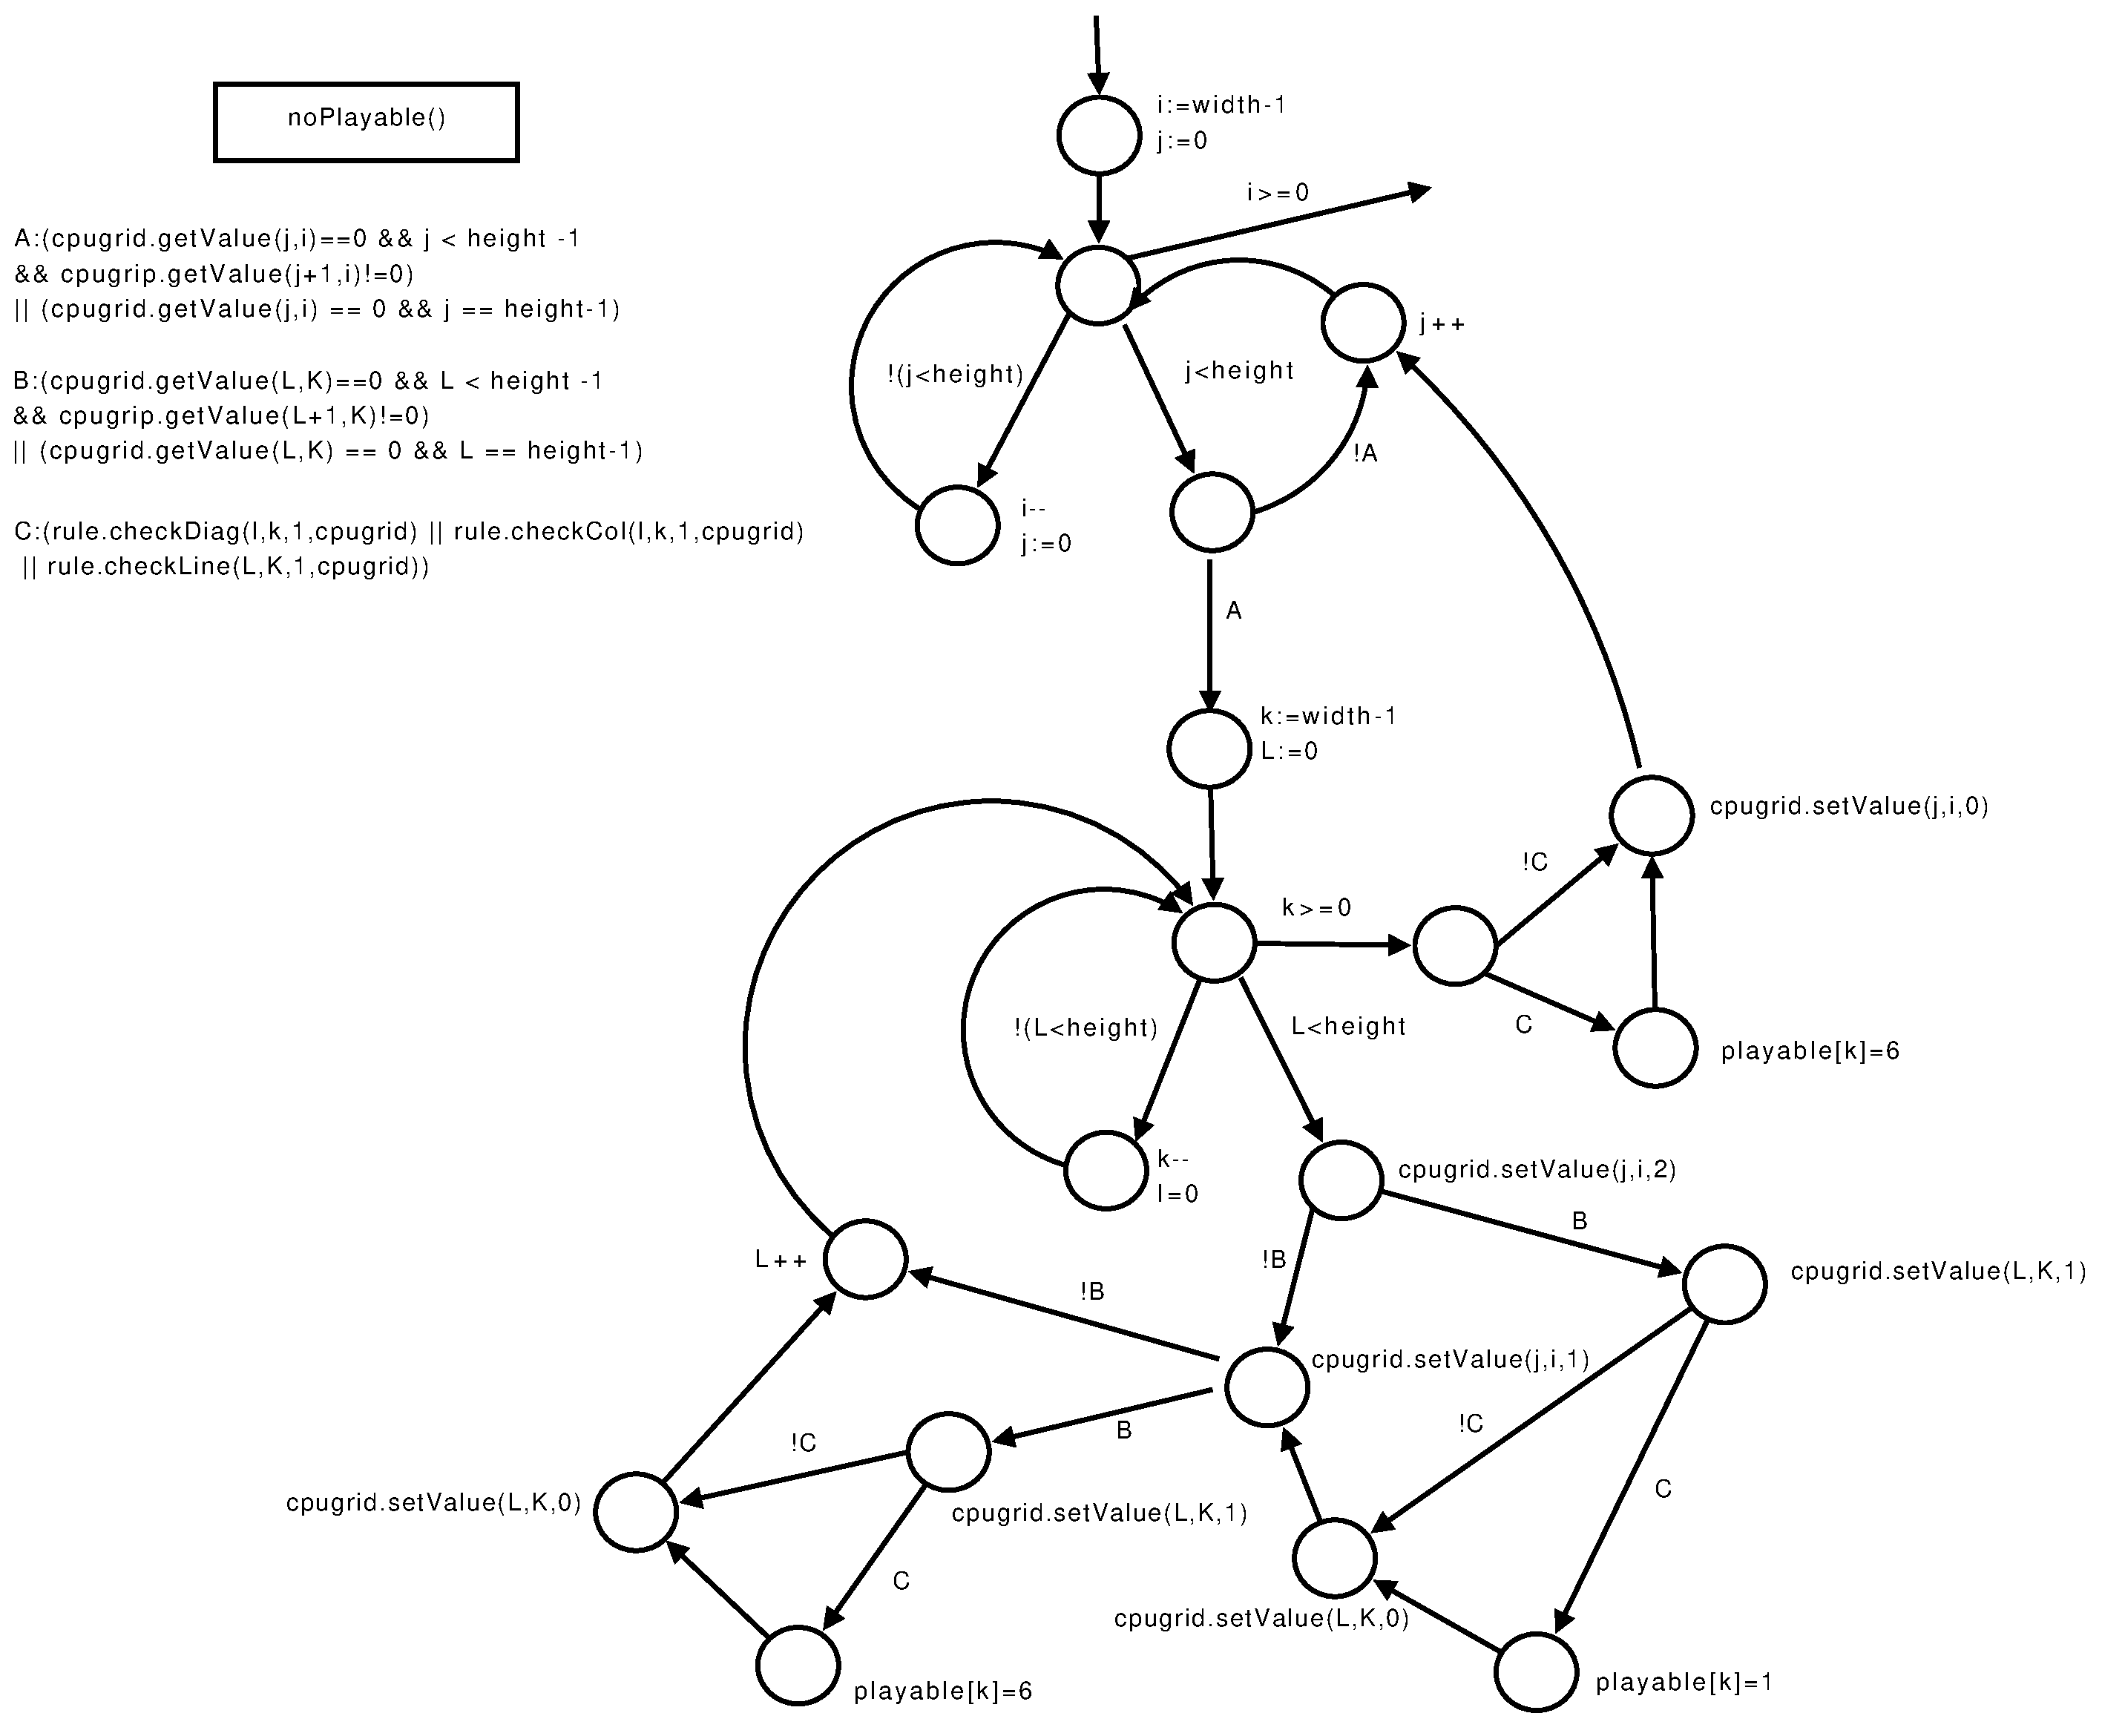
\includegraphics[scale=0.5]{noplayable}
  \caption{Fonction noPlayable}
\end{center}
\end{figure}

\newpage
\texttt{breakStrategy()}\\
\begin{figure}[h]
\begin{center}
  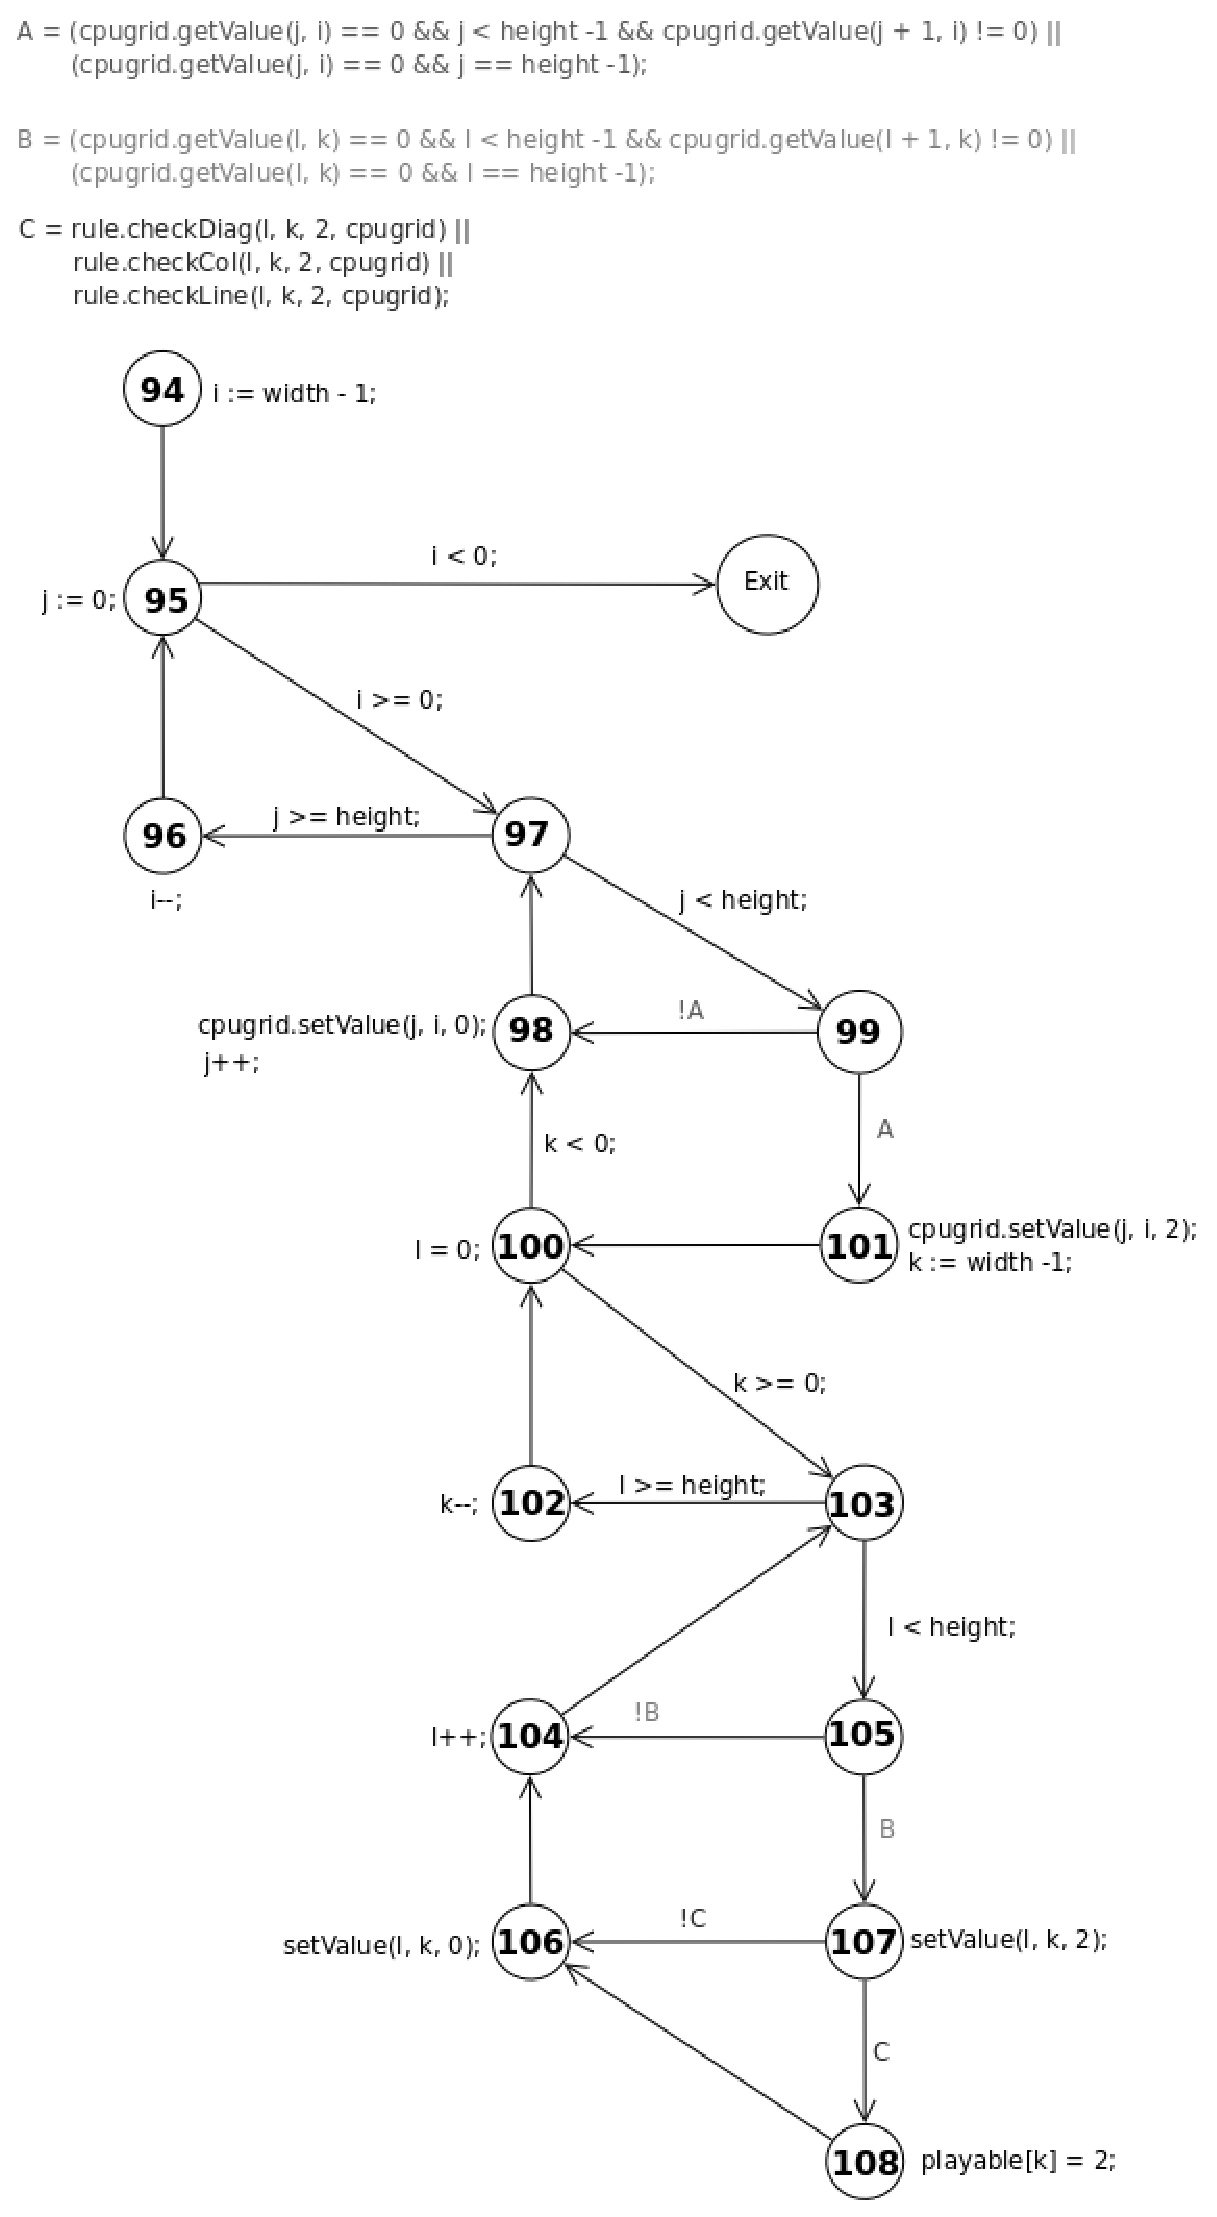
\includegraphics[scale=0.4]{breakStrategy}
  \caption{Fonction breakStrategy}
\end{center}
\end{figure}

\newpage
\texttt{strategy()}\\
\begin{figure}[h]
\begin{center}
  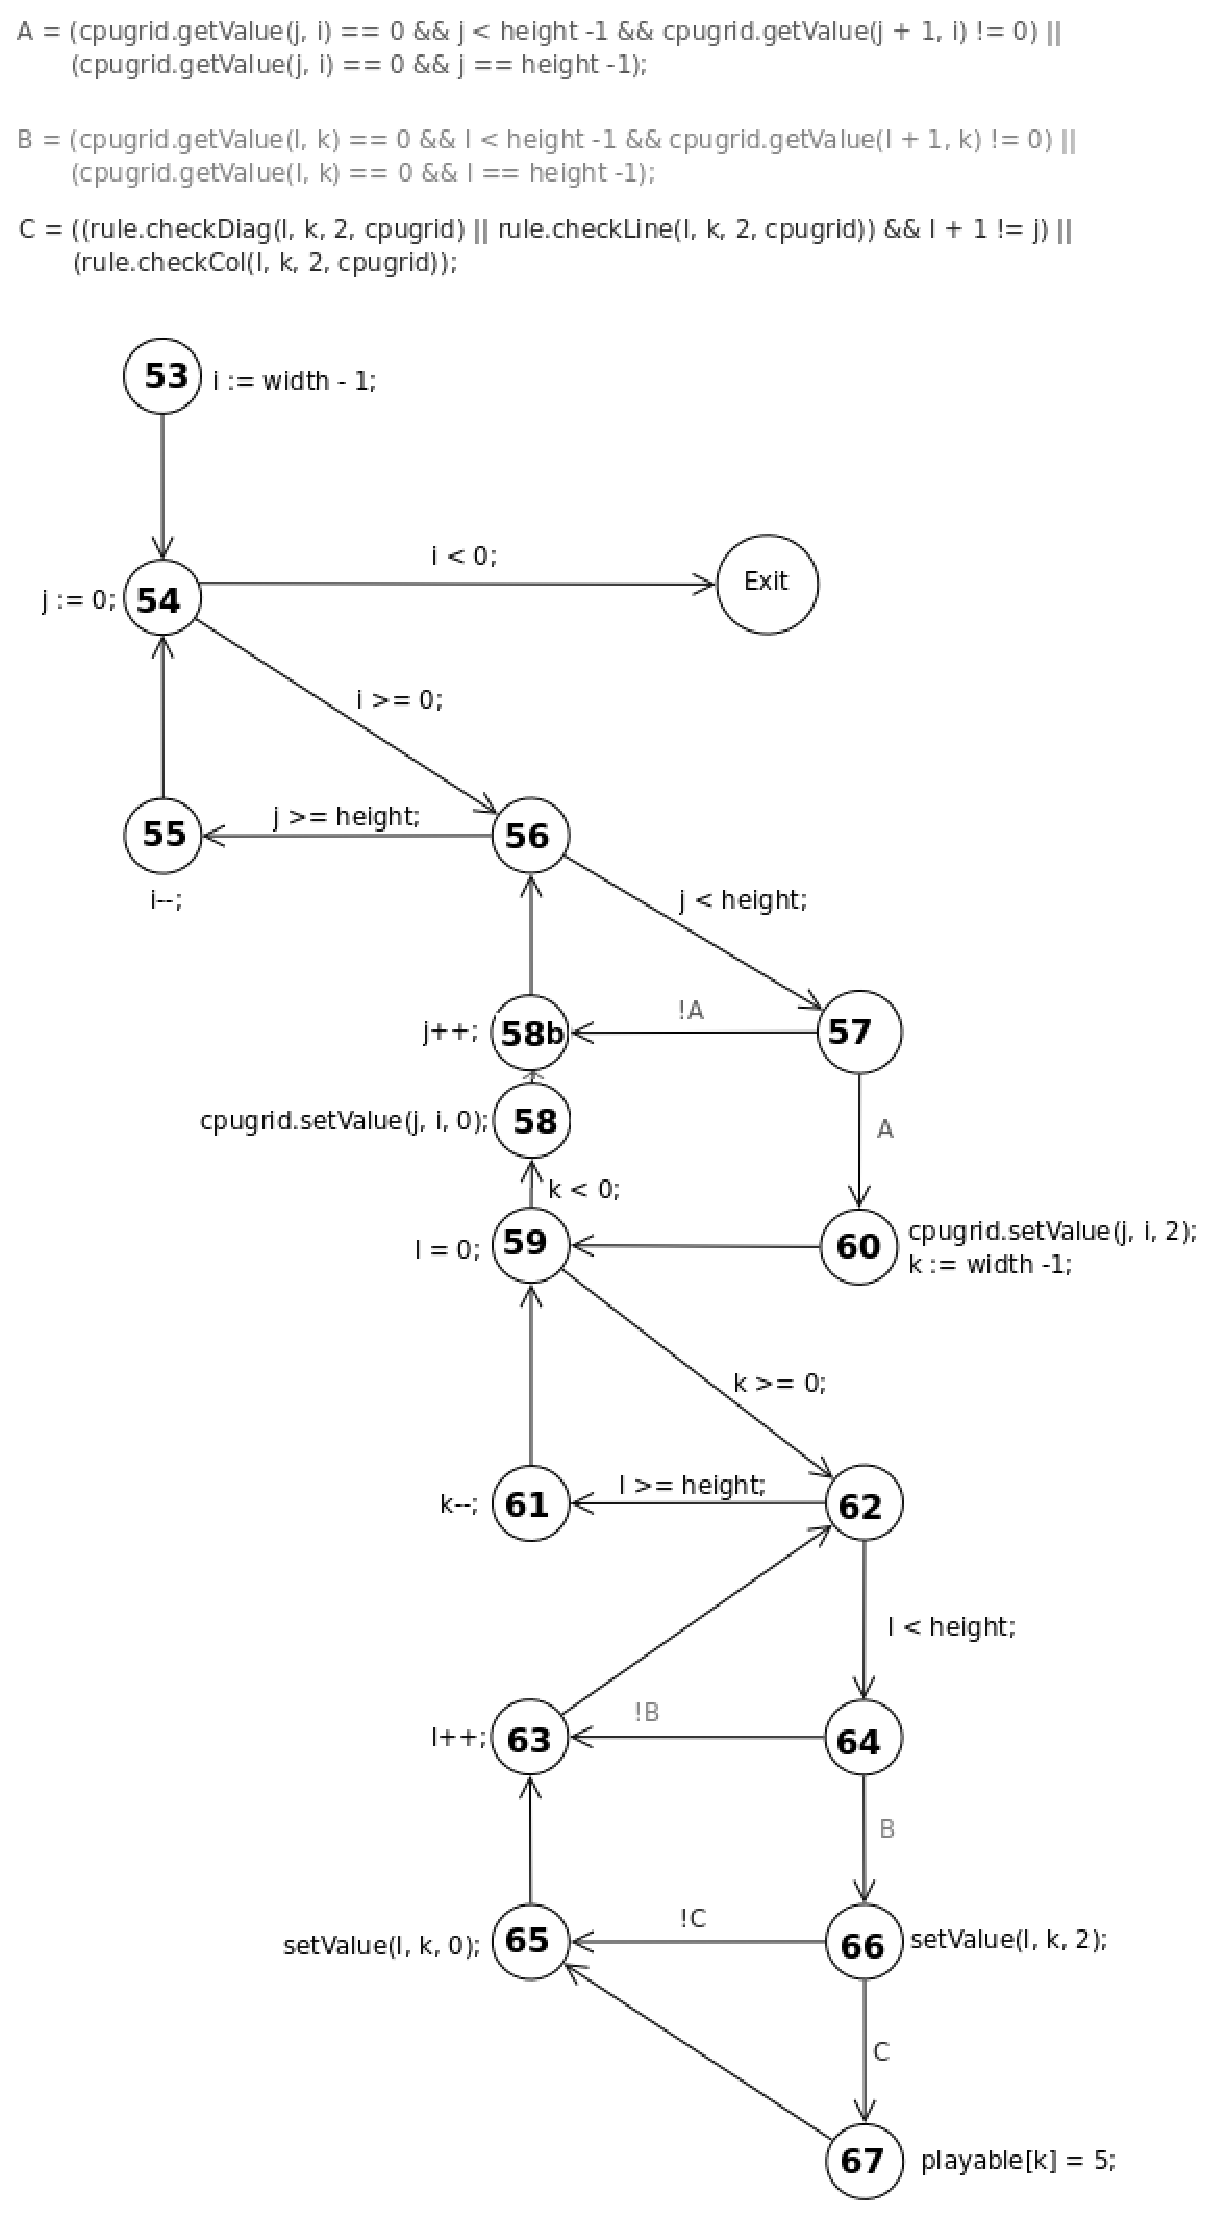
\includegraphics[scale=0.4]{strategy}
  \caption{Fonction figure}
\end{center}
\end{figure}

\section{conclusion analyse statique }

Cette annalyse des CFA nous a permit de trouver des DT avec un pourcentage de
couverture suffisant pour �tre pertinentes. Cela � grandement facilit�
la mise en place d'un start�gie de test efficace des diff�rents
modules du puisssance4. Il est aussi int�ressant de mentioner le fait
que la cr�ation du CFA \texttt{v�rification\_choix()} nous a permit de
corriger une erreur d'�criture de fonction. En effet nous avions cod�
cette fonction de telle fa�on qu'elle nous renvoyait toujours true,
m�me en passant des valeurs qui sortaient des limites de la
grille. Le CFA � mis en valeur ce d�faut de conception et nous �
permit de corriger tr�s t�t ce probl�me. 

\newpage
% -*- mode: latex; coding: latin-1-unix -*- %


\section{R�sultats}

\subsection{Tests de validation}

Nous allons voir ici les r�sultats des tests imagin�s pour s'assurer que le programme obtenu respecte bien les termes pr�cis�s dans la sp�cification.\newline\newline


\subsubsection{R�gles de puissance 4}

\begin{itemize}
\item \texttt{Test 1 : existence des configurations de jeu}\newline\newline
Partie Humain vs Humain : succ�s.\newline
Partie Humain vs Cpu niveau 1 : succ�s.\newline
Partie Humain vs Cpu niveau 2 : succ�s.\newline

\item \texttt{Test 2 : tailles de grilles}\newline

L'instanciation d'une grille 6x7 a �t� r�alis�e � de multiples reprises avec succ�s.\newline

Pour les autres dimensions, nous avons d�cid� de r�aliser une analyse partitionnelle bas�e sur l'agrandissement et la r�duction de la grille d'origine.\newline

Pour �prouver le programme nous avons d�fini une relation d'�quivalence comme tel:\newline
Deux donn�es de tests $dt1$ et $dt2$ (ici des entiers repr�sentant les 2 dimensions de la grille) sont en relation : $dt1 \diamond dt2$ si et seulement si leur valeur appartient au m�me intervalle $I \in N$.\newline
On forme une partition de ces intervalles sur l'ensemble des valeurs logiques d'instantiation $ I_{logique}=[4,+\infty]$. On entend par valeur logique d'instanciation une valeur susceptible d'�tre instanci�e car elle permet de jouer une partie (i.e on n'instanciera jamais une grille de dimensions -1,3 car une valeur n�gative n'a aucun sens et une valeur comprise entre 0 et 4 n'est pas suffisante pour qu'il soit possible de gagner). Voici donc les intervalles concern�s :\newline

On suppose que $dtH$ repr�sente la hauteur de la grille, $dtL$ la largeur. Les valeurs par d�faut �tant $dtH = 6$ et $dtL = 7$, on va s'interesser aux intervalles inf�rieurs et sup�rieurs et lancer les tests sur chaque combinaison des classes d'�quivalences form�es par la m�thode expliqu�e ci-dessus. Ainsi, pour la hauteur, on obtient les intervalles $ I_{H1}=[4,6]$ , $I_{H2}=]6,+\infty]$ et pour la largeur, $I_{L1}=[4,7]$, $I_{H2}=]7,+\infty]$.

On d�termine alors exhaustivement l'ensemble des combinaisons des classes d'�quivalence :\texttt{$(I_{H1}$,$ I_{L1})$},\texttt{$(I_{H2}$,$ I_{L1})$},\texttt{$(I_{H1}$,$ I_{L2})$},\texttt{$(I_{H2}$,$ I_{L2})$}\newline

Enfin, on choisit arbitrairement une $dt$ par classe d'�quivalence et on obtient les 4 jeux de test suivants d�rivant des couples pr�c�dents:
 \texttt{(dtH = 4, dtL = 5)}, \texttt{(dtH = 15, dtL = 6)}, \texttt{(dtH = 5, dtL = 20)}, \texttt{(dtH = 9, dtL = 9)}.

Chacune de ces instantiations a �t� r�alis�e avec succ�s et le comportement du programme correspondait � nos atttentes.\newline \newline

\item \texttt{Test 3 : match nul}\newline
Nous avons jou� une partie de mani�re � obtenir un match nul, un �l�ment de l'interface graphique nous a effectivement averti de cette terminaison.\newline\newline
\end{itemize}

\begin{itemize}
\item \texttt{Test 4 : �chantillon d'utilisateurs}\newline
L'ensemble des �tudiants auquels nous avons soumis le programme ont �t� d'accord pour dire que les r�gles avaient �t� respect�es lors de leur partie.\newline
\end{itemize}

\begin{itemize}
\item \texttt{Test 5 : parties al�atoires}\newline
Nous avons test� avec succ�s la progression et terminaison correcte de dizaines de parties g�n�r�es � l'aide d'un algorithme al�atoire pour le choix du coup � jouer par les 2 joueurs ordinateurs. Cette fonction est accessible en d�marrant le programme avec l'option \texttt{-test}.
\end{itemize}

\subsubsection{Configurations de jeu}

Il suffit d'un test fonctionnel basique dont l'objet est de v�rifier que lorsque le programme est lanc�, les diff�rentes configurations de jeu sont disponibles.\newline\newline

\begin{itemize}
\item \texttt{Test 6 : acc�s aux diff�rentes configurations}\newline
Chacun des boutons de l'interface graphique entra�ne la cr�ation de la partie correspondante. Nous avons v�rifi� exhaustivement chaque bouton.\newline
\end{itemize}

\subsubsection{Types de joueurs}

\begin{itemize}
\item \texttt{Test 7 : deux niveaux de jeu}\newline
De multiples parties avec les 2 niveaux de jeu ont �t� r�alis�es avec succ�s.\newline
\end{itemize}

% -*- mode: latex; coding: latin-1-unix -*- %

\subsection{Tests d'int�gration}

Nous n'avons pas cod� l'interface graphique directement, elle n'est
venue que dans un second temps. Autrement dit pour jouer au puissance
4 on passait par la console.

Mais avant d�n arriv� la nous avons int�gr� notre \texttt{GameEngine}
avec notre \texttt{DataStructure}.

La simplicit�, � ce moment, de ces deux m�thodes �taient telles, que les
tests d'int�grations ne nous ont pas vraiment permis, � ce moment l�,
d'am�liorer le code.

Dans un second temps, nous avons cr�� un module \texttt{Rule} que nous
avons int�gr� � notre \texttt{GameEngine}. Nous avons rencontr� de
nombreux probl�mes. Car notre \texttt{Rule} a besoin de la grille pour
pouvoir v�rifier si la grille est valide et surtout si il y a un
gagnant. Pour cela nous avons du cr�er des accesseurs pour les
variables \texttt{private} de \texttt{DataStructure}.

L'�tape d'apr�s nous avons mis en place un joueur qui jouait � travers
la console. Encore une fois dans un soucis de tests d'int�grations
pour v�rifier l'affichage (primaire) de la grille dans notre
console. Cette �tape nous a permis de voir plusieurs choses.
\bigskip
\begin{itemize}
\item D�rouler le jeu en s�quence\newline
Il fallait savoir qui jouait et donc alterner les deux joueurs.
\bigskip
\item D�terminer la fin du jeu\newline
Il fallait faire des appels ing�nieux � \texttt{Rule} pour d�terminer
si il y a un vainqueur, mais aussi si la partie est termin�e, match
nul. Pour ce dernier cas, nous avons choisi la solution de
facilit�. Nous avons mis en place un compteur dans le GameEngine, qui
compte le nombre de coup jou�. Et si ce compteur atteint la dimension
de la matrice, alors ca veut dire que chaque case de la grille a �t�
modifi�e au moins une fois.
\bigskip
\item V�rifier la validit� du coup jou�\newline
Ca n'a pas vraiment �t� ca qui nous a pos� probl�me, mais plut�t le
fait que si nous jouions mal il fallait refaire jouer le m�me joueur
et ne pas incr�menter le compteur. La seconde partie de la derniere
phrase ne nous a pas parue �vidente, c'est pourquoi nous avons du
tester plusieurs cas. 

\bigskip
\begin{itemize}
\item Les deux joueurs jouent toujours correctement et
un des gagnent.
\item Les deux joueurs jouent toujours correctement mais ca fini par
  un match nul
\item Les deux joueurs ne jouent pas correctement et il y avait match nul
\end{itemize}
\end{itemize}
Ce dernier test nous a permis de voir que nous avions fait une bourde
au niveau du compteur, qui fut corrig� sur l'instant.

\bigskip
A ce niveau d'int�gration l�, le programme fonctionnait
correctement. On pouvait jouer au puissance 4 a deux joueurs sans
probl�me. L'�tape suivante a consist� � mettre ne place une interface
graphique. D'apr�s le sujet cette interface graphique doit etre
interchangeable en ne modifiant qu'une seule ligne de code dans notre
\texttt{GameEngine}.
Pour respecter cette r�gle, nous avons mis une interface dont notre
interface graphique h�rite. Ca nous a fait remanipuler notre
architecture, mais cela correspondait d�j� en partie mieux au sujet.

Notre interface graphique est assez rudimentaire, les tests qui ont
�t� effectu�s ont �t� basique. Nous avons effectu� les m�mes tests que
lors de l'int�gration de l'affichage console. Mais nous avons d�duits
de grosse am�liorations sur le \texttt{GameEngine}. C'est lors de ces
tests que nous avons ajout� les m�thodes qui servent a griser les
boutons qui correspondent a des colonnes pleines. Ainsi que les
fonctionnalit� qui consistait a ajouter le nom du vainqueur sur notre
grille, mais �galement la possibilit� de faire un reset (et cette fois
on a pens� a remettre � z�ro le compteur).
Nous avons quand m�me d�tect� des bug, dont la source nous est encore
inconnue mais que nous avons corrig� en ajoutant un
\texttt{System.out.println();}. Car notre affichage ne fonctionnait
pas sans ca. Il est possible d'am�liorer cette partie en mettant un
simple \texttt{System.out.flush()}, mais ca reste a tester.

En int�grant notre intelligence artificelle nous avons du modifier le
\texttt{GameEngine} qui avait une m�thode \texttt{start()} pour chaque
\texttt{mode} (0, 1 et 2). L'intelligence artificelle s�st faite assez
ais�ment, car elle se sert de \texttt{Rule} et du'une
\texttt{DataStructure}. Lors de l'int�gration de notre intelligence
artificelle, le \texttt{GameEngine} �tait suffisament robuste pour
r�pondre a des cas d'erreurs, pr�c�demment test� lors de l'int�gration
du mode console.
Cependant,pour ajouter une intelligence artificielle il fallait
modifier les classes \texttt{GameEngine} et \texttt{IAFourInARow} ce
qui ne crrespondait aucunement au sujet. Sur ce point nous avons du
faire des efforts d'architecture.

En cr�ant une interface \texttt{Player} nous pouvions instancier un
joueur humain ou un ordinateur. Si c'�tait un ordinateur on
instanciait un \texttt{IAFourInARow} et ca ne r�pondait pas � nos
besoin lors de l'int�gration.

Nous avons du remodifier le code et cr�er une nouvelle interface
\texttt{Cpu} dont le but �tait de permettre l'int�gration d'une
nouvelle intelligence artificielle en ne modifiant qu'une seule ligne
de code. Ca a apport� une modificaiton simple et �vidente sur notre
\texttt{CpuPlayer}.

Avant on faisait :\newline
\texttt{IAFourInARow() cpu1 = new IAFourInARow();}

Maintenant on fait :\newline
\texttt{Cpu() cpu1 = new IAFourInARow();}

Le gros changement fut de faire impl�ment� \texttt{IAFourInARow} a
notre interface \texttt{Cpu}.

Une fois cette modification apport�, on avait un code modulaire pour
l'interface graphique et pour l'ordinateur. On a donc fait un peu de
z�le en faisant de m�me pour \texttt{Rule} qui est devenue
\texttt{FourInARowRule} et qui impl�mente l'interface \texttt{Rule}.

De cette mani�re on peut jouer a plusieurs jeux en changeant de r�gle
(Puissance 5 par exemple).

% -*- mode: latex; coding: latin-1-unix -*- %

\subsection{Tests Unitaires}

\subsubsection{DataStructureTest}

La plupart des bugs identifi�s seront li�s aux valeurs des positions de la grille.\newline
Particuli�rement, une affectation d'une couleur � une position \textbf{hors limite} est source 
de bugs.\newline
Le fait d'affecter une couleur quelconque � la position \textbf{(0,9)} d'une grille (8,9) est typiquement le type de bugs qu'on aura � traiter.

\paragraph{Test 1} - R�sultats

\begin{verbatim}
    public void testInvalidSetValues() {
        assertFalse(matrix.setValue(10, 1, 0));
        assertFalse(matrix.setValue(1, 10, 1));
        assertFalse(matrix.setValue(10, 10, 2));
    }
\end{verbatim}
   
Ce test montre bien qu'il n'est pas possible d'affecter des couleurs \textbf{hors des limites} 
� la grille \textbf{matrix} (6,7) consid�r�e.

\paragraph{Test 2} - R�sultats

\begin{verbatim}
    public void testNegativeMatrix() {
        int resultNH = negative_matrix.getHeight();
        assertEquals("la hauteur d'une negative_matrix n'est pas  6", resultNH, 6);

        int resultNW = negative_matrix.getWidth();
        assertEquals("la largeur d'une negative_matrix n'est pas  6", resultNW, 7);
   }    
\end{verbatim}

Ce test montre que les param�tres (height , width) d'une grille "n�gative" n'ont 
de valeur que respectivement 6(hauteur) et 7(largeur).  \newline
Ce m�me type de test sera experiment� sur une grille "zero" et donnera le m�me r�sultat.

\paragraph{Test 3} - R�sultats

\bigskip
Tester \textbf{aux limites} la possiblit� d'affecter des couleurs � une grille (6,7).\newline
Ce test peut �tre g�n�ralis� � des grilles (i,j) avec i>0 et j>0.\newline  

En effet, l'affectation des couleurs dans le Domaine des positions [0...42] r�ussit avec succ�s.
Mais, pour les valeurs -1 et 43 le test montre une impossibilit� d'affectation.\newline

\subsubsection{IAfourInARowTest}

Ces tests nous ont permis de r�v�ler de nombreux bugs li�s aux comportements des IA. Tout d'abord sur les strat�gies de \texttt{playable[]} qui n'�taient pas toujours juste par rapport � l'�tat actuel de la grille,et aussi la fa�on de jouer des IA ne correspondaient pas toujours � ce qui �tait attendu d� au fait des priorit�s des \texttt{playable}.

Pour chaque �tat de la grille il nous �tait possible � l'aide de l'algorithme de conna�tre l'�tat de \texttt{playable[]} et le coup que doit jouer l'IA ainsi nous avons corrig� les moteurs d'IA pour qu'ils nous donnent exactement les r�sultats escompt�s dans les cas typiques ci-dessus.



\subsubsection{FouInRowTest}

La victoire d'un joueur est conditionn�e par le fait qu'un joueur
aligne 4 jetons sur la m�me ligne, colonne ou diagonale. Ceci sera
test� au moyen des 3 m�thodes \texttt{testCheckLine()},
\texttt{testCheckCol()} et \texttt{testCheckDiag()}. Le r�sultat
obtenu sera satisfaisant � la fois pour les tests d'alignement et
celui de la jouabilit� d'un coup donn�.(cf 4.4.2)\newline


\subsubsection{GameEngineTest}


Tester le moteur de jeu, nous permettra de v�rifier correctement que
les modes initialement initialis�s seront valides. Et dans un deuxi�me
temps, de tester les diff�rents cas de figure de fin de
partie.\newline

Dans ce dernier point, les possibilit�s sont multiples et quelque unes
d'entres elles seront test�s(cf 4.5.2). \newline
Mais, nous avons determin� tout de m�me un cas de figure non trait� et
impossible � tester vu l'�tat actuelle de notre code, donc un bug li�
� notre impl�mentation.\newline
C'est lorsqu'un joueur joue le dernier coup de la partie(grille
remplie compl�tement) et aligne 4 jetons suite � ce m�me coup,
on est incapable de d�signer le vainqueur comme �tant celui qui a jou�
en dernier.\newline


\newpage

\section{conclusion}


La simplicité du support Puissance 4 nous a permis de ne pas nous focaliser sur des problèmes de réalisation. Nous avons ainsi pu prendre du temps pour développer une stratégie de test ou du moins une série de tests et tenter d'aborder les différents outils et phases vus en cours. Nous nous sommes d'efforcés de couvrir une variété de tests aussi large que possible. Ainsi, on peut observer des tests classiques que des tests unitaires réalisés à l'aide de JUnit ou des parcours de chemins du programme basés sur une analyse statique. Le nombre de participants au projet n'a pas toujours facilité notre organisation puisqu'il était difficile d'organiser des réunions au travers de nos examens de Janvier. Nous estimons cependant que le code a atteint une certaine maturité et que le rapport regroupe une quantité convenable d'informations au regard du travail effectué.

\end{document}
